% Options for packages loaded elsewhere
\PassOptionsToPackage{unicode}{hyperref}
\PassOptionsToPackage{hyphens}{url}
%
\documentclass[
]{book}
\usepackage{amsmath,amssymb}
\usepackage{lmodern}
\usepackage{iftex}
\ifPDFTeX
  \usepackage[T1]{fontenc}
  \usepackage[utf8]{inputenc}
  \usepackage{textcomp} % provide euro and other symbols
\else % if luatex or xetex
  \usepackage{unicode-math}
  \defaultfontfeatures{Scale=MatchLowercase}
  \defaultfontfeatures[\rmfamily]{Ligatures=TeX,Scale=1}
\fi
% Use upquote if available, for straight quotes in verbatim environments
\IfFileExists{upquote.sty}{\usepackage{upquote}}{}
\IfFileExists{microtype.sty}{% use microtype if available
  \usepackage[]{microtype}
  \UseMicrotypeSet[protrusion]{basicmath} % disable protrusion for tt fonts
}{}
\makeatletter
\@ifundefined{KOMAClassName}{% if non-KOMA class
  \IfFileExists{parskip.sty}{%
    \usepackage{parskip}
  }{% else
    \setlength{\parindent}{0pt}
    \setlength{\parskip}{6pt plus 2pt minus 1pt}}
}{% if KOMA class
  \KOMAoptions{parskip=half}}
\makeatother
\usepackage{xcolor}
\IfFileExists{xurl.sty}{\usepackage{xurl}}{} % add URL line breaks if available
\IfFileExists{bookmark.sty}{\usepackage{bookmark}}{\usepackage{hyperref}}
\hypersetup{
  pdftitle={Cours d'Analyse de Données avec R},
  pdfauthor={Priestley},
  hidelinks,
  pdfcreator={LaTeX via pandoc}}
\urlstyle{same} % disable monospaced font for URLs
\usepackage{color}
\usepackage{fancyvrb}
\newcommand{\VerbBar}{|}
\newcommand{\VERB}{\Verb[commandchars=\\\{\}]}
\DefineVerbatimEnvironment{Highlighting}{Verbatim}{commandchars=\\\{\}}
% Add ',fontsize=\small' for more characters per line
\usepackage{framed}
\definecolor{shadecolor}{RGB}{248,248,248}
\newenvironment{Shaded}{\begin{snugshade}}{\end{snugshade}}
\newcommand{\AlertTok}[1]{\textcolor[rgb]{0.94,0.16,0.16}{#1}}
\newcommand{\AnnotationTok}[1]{\textcolor[rgb]{0.56,0.35,0.01}{\textbf{\textit{#1}}}}
\newcommand{\AttributeTok}[1]{\textcolor[rgb]{0.77,0.63,0.00}{#1}}
\newcommand{\BaseNTok}[1]{\textcolor[rgb]{0.00,0.00,0.81}{#1}}
\newcommand{\BuiltInTok}[1]{#1}
\newcommand{\CharTok}[1]{\textcolor[rgb]{0.31,0.60,0.02}{#1}}
\newcommand{\CommentTok}[1]{\textcolor[rgb]{0.56,0.35,0.01}{\textit{#1}}}
\newcommand{\CommentVarTok}[1]{\textcolor[rgb]{0.56,0.35,0.01}{\textbf{\textit{#1}}}}
\newcommand{\ConstantTok}[1]{\textcolor[rgb]{0.00,0.00,0.00}{#1}}
\newcommand{\ControlFlowTok}[1]{\textcolor[rgb]{0.13,0.29,0.53}{\textbf{#1}}}
\newcommand{\DataTypeTok}[1]{\textcolor[rgb]{0.13,0.29,0.53}{#1}}
\newcommand{\DecValTok}[1]{\textcolor[rgb]{0.00,0.00,0.81}{#1}}
\newcommand{\DocumentationTok}[1]{\textcolor[rgb]{0.56,0.35,0.01}{\textbf{\textit{#1}}}}
\newcommand{\ErrorTok}[1]{\textcolor[rgb]{0.64,0.00,0.00}{\textbf{#1}}}
\newcommand{\ExtensionTok}[1]{#1}
\newcommand{\FloatTok}[1]{\textcolor[rgb]{0.00,0.00,0.81}{#1}}
\newcommand{\FunctionTok}[1]{\textcolor[rgb]{0.00,0.00,0.00}{#1}}
\newcommand{\ImportTok}[1]{#1}
\newcommand{\InformationTok}[1]{\textcolor[rgb]{0.56,0.35,0.01}{\textbf{\textit{#1}}}}
\newcommand{\KeywordTok}[1]{\textcolor[rgb]{0.13,0.29,0.53}{\textbf{#1}}}
\newcommand{\NormalTok}[1]{#1}
\newcommand{\OperatorTok}[1]{\textcolor[rgb]{0.81,0.36,0.00}{\textbf{#1}}}
\newcommand{\OtherTok}[1]{\textcolor[rgb]{0.56,0.35,0.01}{#1}}
\newcommand{\PreprocessorTok}[1]{\textcolor[rgb]{0.56,0.35,0.01}{\textit{#1}}}
\newcommand{\RegionMarkerTok}[1]{#1}
\newcommand{\SpecialCharTok}[1]{\textcolor[rgb]{0.00,0.00,0.00}{#1}}
\newcommand{\SpecialStringTok}[1]{\textcolor[rgb]{0.31,0.60,0.02}{#1}}
\newcommand{\StringTok}[1]{\textcolor[rgb]{0.31,0.60,0.02}{#1}}
\newcommand{\VariableTok}[1]{\textcolor[rgb]{0.00,0.00,0.00}{#1}}
\newcommand{\VerbatimStringTok}[1]{\textcolor[rgb]{0.31,0.60,0.02}{#1}}
\newcommand{\WarningTok}[1]{\textcolor[rgb]{0.56,0.35,0.01}{\textbf{\textit{#1}}}}
\usepackage{longtable,booktabs,array}
\usepackage{calc} % for calculating minipage widths
% Correct order of tables after \paragraph or \subparagraph
\usepackage{etoolbox}
\makeatletter
\patchcmd\longtable{\par}{\if@noskipsec\mbox{}\fi\par}{}{}
\makeatother
% Allow footnotes in longtable head/foot
\IfFileExists{footnotehyper.sty}{\usepackage{footnotehyper}}{\usepackage{footnote}}
\makesavenoteenv{longtable}
\usepackage{graphicx}
\makeatletter
\def\maxwidth{\ifdim\Gin@nat@width>\linewidth\linewidth\else\Gin@nat@width\fi}
\def\maxheight{\ifdim\Gin@nat@height>\textheight\textheight\else\Gin@nat@height\fi}
\makeatother
% Scale images if necessary, so that they will not overflow the page
% margins by default, and it is still possible to overwrite the defaults
% using explicit options in \includegraphics[width, height, ...]{}
\setkeys{Gin}{width=\maxwidth,height=\maxheight,keepaspectratio}
% Set default figure placement to htbp
\makeatletter
\def\fps@figure{htbp}
\makeatother
\setlength{\emergencystretch}{3em} % prevent overfull lines
\providecommand{\tightlist}{%
  \setlength{\itemsep}{0pt}\setlength{\parskip}{0pt}}
\setcounter{secnumdepth}{5}
\usepackage{booktabs}
\usepackage{tcolorbox}

\newtcolorbox{blackbox}{
  colback=black,
  colframe=orange,
  coltext=white,
  boxsep=5pt,
  arc=4pt}
  
\newtcolorbox{redbox}{
  colback=red,
  colframe=black,
  coltext=white,
  boxsep=5pt,
  arc=4pt}

\newenvironment{infobox}[1]
  {
  \begin{itemize}
  \renewcommand{\labelitemi}{
    \raisebox{-.7\height}[0pt][0pt]{
      {\setkeys{Gin}{width=3em,keepaspectratio}
        
\includegraphics{images/danger.png}}
    }
  }
  \setlength{\fboxsep}{1em}
  \begin{blackbox}
  \item
  }
  {
  \end{blackbox}
  \end{itemize}
  }
  
  
\ifLuaTeX
  \usepackage{selnolig}  % disable illegal ligatures
\fi
\usepackage[]{natbib}
\bibliographystyle{plainnat}

\title{Cours d'Analyse de Données avec R}
\author{Priestley}
\date{2022-04-22}

\begin{document}
\maketitle

{
\setcounter{tocdepth}{1}
\tableofcontents
}
\hypertarget{premier-contact}{%
\chapter{Premier contact}\label{premier-contact}}

Une fois RStudio lancé, vous devriez obtenir une fenêtre similaire à la figure ci-après.

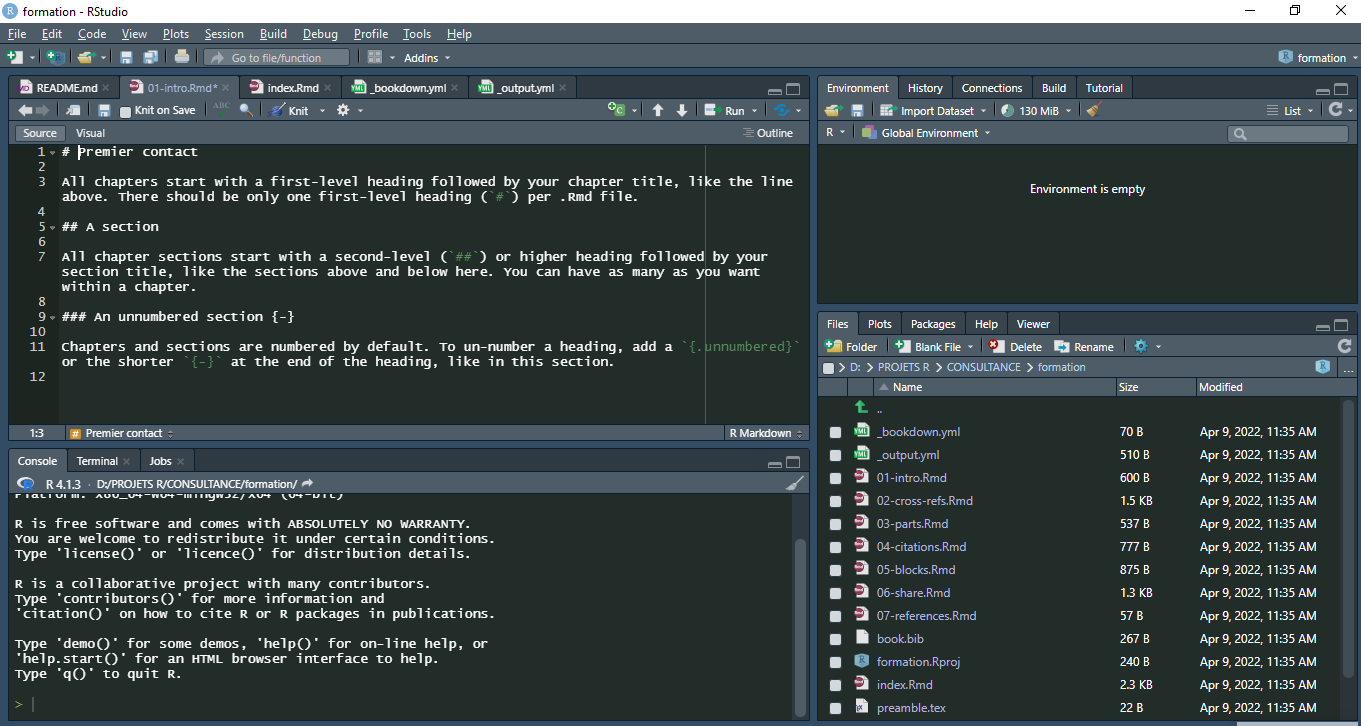
\includegraphics[width=1\linewidth]{images/Capture}
L'interface de RStudio est divisée en quatre quadrants :

\begin{itemize}
\tightlist
\item
  le quadrant supérieur gauche est dédié aux différents fichiers de travail (nous y reviendrons dans le chapitre Premier travail avec les données) ;
\item
  le quadrant inférieur gauche correspond à ce que l'on appelle la console, c'est-à-dire à R proprement dit ;
\item
  le quadrant supérieur droit permet de connaître
  la liste des objets en mémoire ou environnement de travail (onglet Environment)
  ainsi que l'historique des commandes saisies dans la console (onglet History) ;
\item
  le quadrant inférieur droit affiche
  la liste des fichiers du répertoire de travail (onglet Files),
  les graphiques réalisés (onglet Plots),
  la liste des extensions disponibles (onglet Packages),
  l'aide en ligne (onglet Help)
  et un Viewer utilisé pour visualiser certains types de graphiques au format web.
  Inutile de tout retenir pour le moment. Nous aborderons chaque outil en temps utile. Pour l'heure, concentrons-nous sur la console, c'est-à-dire le quadrant inférieur gauche
\end{itemize}

\hypertarget{linvite-de-commandes}{%
\section{L'invite de commandes}\label{linvite-de-commandes}}

Au démarrage, la console contient un petit texte de bienvenue ressemblant à peu près à ce qui suit :

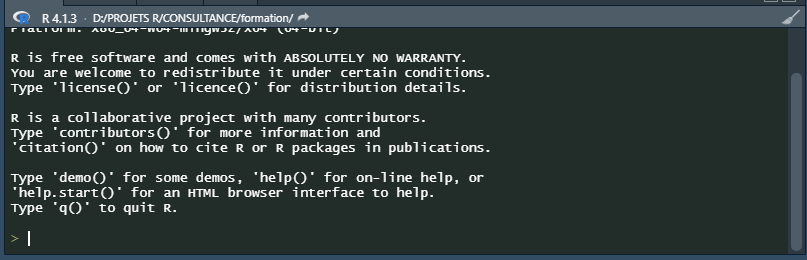
\includegraphics[width=1\linewidth]{images/console}
suivi d'une ligne commençant par le caractère \textgreater{} et sur laquelle devrait se trouver votre curseur. Cette ligne est appelée l'invite de commande (ou prompt en anglais). Elle signifie que R est disponible et en attente de votre prochaine commande.

Nous allons tout de suite lui fournir une première commande. Tapez 2 + 3 dans la console et validez avec la touche Entrée.

\begin{Shaded}
\begin{Highlighting}[]
\DecValTok{2}\SpecialCharTok{+}\DecValTok{3}
\end{Highlighting}
\end{Shaded}

\begin{verbatim}
## [1] 5
\end{verbatim}

En premier lieu, vous pouvez noter la convention typographique utilisée dans ce documents. Les commandes saisies dans la console sont indiquées sur un fond gris et précédé de R\textgreater. Le résultat renvoyé par R est quant à lui affiché juste en-dessous sur fond blanc.

Bien, nous savons désormais que R sait faire les additions à un chiffre. Nous pouvons désormais continuer avec d'autres opérations arithmétiques de base :

\begin{Shaded}
\begin{Highlighting}[]
\DecValTok{8{-}4}
\end{Highlighting}
\end{Shaded}

\begin{verbatim}
## [1] 4
\end{verbatim}

\begin{Shaded}
\begin{Highlighting}[]
\DecValTok{14}\SpecialCharTok{*}\DecValTok{5}
\end{Highlighting}
\end{Shaded}

\begin{verbatim}
## [1] 70
\end{verbatim}

\begin{Shaded}
\begin{Highlighting}[]
\SpecialCharTok{{-}}\DecValTok{3}\SpecialCharTok{/}\DecValTok{10}
\end{Highlighting}
\end{Shaded}

\begin{verbatim}
## [1] -0.3
\end{verbatim}

\begin{Shaded}
\begin{Highlighting}[]
\SpecialCharTok{{-}}\FloatTok{0.3}
\end{Highlighting}
\end{Shaded}

\begin{verbatim}
## [1] -0.3
\end{verbatim}

On remarquera que R est anglo-saxon. Les nombres sont donc saisies « à l'anglaise », c'est-à-dire en utilisant le point (.) comme séparateur pour les décimales.
Une petite astuce très utile lorsque vous tapez des commandes directement dans la console : en utilisant les flèches Haut et Bas du clavier, vous pouvez naviguer dans l'historique des commandes tapées précédemment. Vous pouvez alors facilement réexécuter ou modifier une commande particulière.

Sous RStudio, l'onglet History du quadrant haut-droite vous permet de consulter l'historique des commandes que vous avez transmises à R.

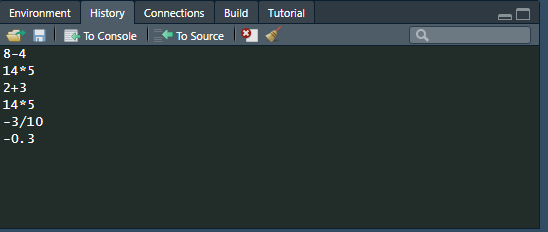
\includegraphics[width=1\linewidth]{images/history}

\hypertarget{des-objets}{%
\section{Des objets}\label{des-objets}}

\hypertarget{objets-simples}{%
\subsection{Objets simples}\label{objets-simples}}

Faire des opérations arithmétiques, c'est bien, mais sans doute pas totalement suffisant. Notamment, on aimerait pouvoir réutiliser le résultat d'une opération sans avoir à le resaisir ou à le copier/coller.

Comme tout langage de programmation, R permet de faire cela en utilisant des objets. Prenons tout de suite un exemple :

\begin{Shaded}
\begin{Highlighting}[]
\NormalTok{x }\OtherTok{\textless{}{-}} \DecValTok{2}
\end{Highlighting}
\end{Shaded}

Que signifie cette commande ? L'opérateur \textless- est appelé opérateur d'assignation. Il prend une valeur quelconque à droite et la place dans l'objet indiqué à gauche. La commande pourrait donc se lire mettre la valeur 2 dans l'objet nommé x.
NB:Il existe trois opérateurs d'assignation sous R. Ainsi les trois écritures suivantes sont équivalentes :

\begin{Shaded}
\begin{Highlighting}[]
\NormalTok{x }\OtherTok{\textless{}{-}} \DecValTok{2}
\NormalTok{x }\OtherTok{=} \DecValTok{2}
\DecValTok{2} \OtherTok{{-}\textgreater{}}\NormalTok{ x}
\end{Highlighting}
\end{Shaded}

Cependant, pour une meilleure lecture du code, il est conseillé de n'utiliser que \textless-. Ainsi, l'objet créé est systématiquement affiché à gauche. De plus, le symbole = sert également pour écrire des conditions ou à l'intérieur de fonctions. Il est donc préférable de ne pas l'utiliser pour assigner une valeur (afin d'éviter les confusions).
On va ensuite pouvoir réutiliser cet objet dans d'autres calculs ou simplement afficher son contenu :

\begin{Shaded}
\begin{Highlighting}[]
\NormalTok{x}\SpecialCharTok{+}\DecValTok{3}
\end{Highlighting}
\end{Shaded}

\begin{verbatim}
## [1] 5
\end{verbatim}

On peut utiliser autant d'objets qu'on veut. Ceux-ci peuvent contenir des nombres, des chaînes de caractères (indiquées par des guillemets droits doubles '' ou simples ') et bien d'autres choses encore :

\begin{Shaded}
\begin{Highlighting}[]
\NormalTok{x }\OtherTok{\textless{}{-}} \DecValTok{27}
\NormalTok{y }\OtherTok{\textless{}{-}} \DecValTok{10}
\NormalTok{foo }\OtherTok{\textless{}{-}}\NormalTok{ x }\SpecialCharTok{+}\NormalTok{ y}
\NormalTok{foo}
\end{Highlighting}
\end{Shaded}

\begin{verbatim}
## [1] 37
\end{verbatim}

\begin{Shaded}
\begin{Highlighting}[]
\NormalTok{x }\OtherTok{\textless{}{-}} \StringTok{"Hello"}
\NormalTok{foo }\OtherTok{\textless{}{-}}\NormalTok{ x}
\NormalTok{foo}
\end{Highlighting}
\end{Shaded}

\begin{verbatim}
## [1] "Hello"
\end{verbatim}

Les noms d'objets peuvent contenir des lettres, des chiffres, les symboles . et \_. Ils doivent impérativement commencer par une lettre (jamais par un chiffre). R fait la différence entre les majuscules et les minuscules, ce qui signifie que x et X sont deux objets différents. On évitera également d'utiliser des caractères accentués dans les noms d'objets. Comme les espaces ne sont pas autorisés on pourra les remplacer par un point ou un tiret bas.

Enfin, signalons que certains noms courts sont réservés par R pour son usage interne et doivent être évités. On citera notamment c, q, t, C, D, F, I, T, max, min\ldots{}

Dans RStudio, l'onglet Environment dans le quadrant supérieur droit indique la liste des objets que vous avez précédemment créés, leur type et la taille qu'ils occupent en mémoire.

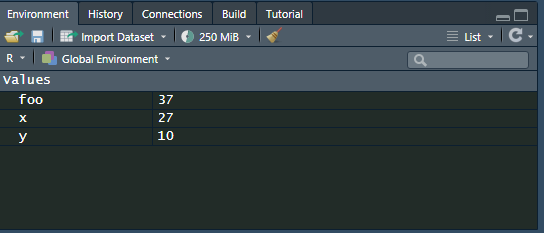
\includegraphics[width=1\linewidth]{images/environement}

\hypertarget{vecteurs}{%
\subsection{Vecteurs}\label{vecteurs}}

Imaginons maintenant que nous avons interrogé dix personnes au hasard dans la rue et que nous avons relevé pour chacune d'elle sa taille en centimètres. Nous avons donc une série de dix nombres que nous souhaiterions pouvoir réunir de manière à pouvoir travailler sur l'ensemble de nos mesures.

Un ensemble de données de même nature constituent pour R un vecteur (en anglais vector) et se construit à l'aide d'une fonction nommée c.~On l'utilise en lui donnant la liste de nos données, entre parenthèses, séparées par des virgules :

\begin{Shaded}
\begin{Highlighting}[]
\NormalTok{tailles }\OtherTok{\textless{}{-}} \FunctionTok{c}\NormalTok{(}\DecValTok{167}\NormalTok{, }\DecValTok{192}\NormalTok{, }\DecValTok{173}\NormalTok{, }\DecValTok{174}\NormalTok{, }\DecValTok{172}\NormalTok{, }\DecValTok{167}\NormalTok{, }\DecValTok{171}\NormalTok{, }\DecValTok{185}\NormalTok{, }\DecValTok{163}\NormalTok{, }\DecValTok{170}\NormalTok{)}
\end{Highlighting}
\end{Shaded}

Ce faisant, nous avons créé un objet nommé tailles et comprenant l'ensemble de nos données, que nous pouvons afficher en saisissant simplement son nom :

\begin{Shaded}
\begin{Highlighting}[]
\FunctionTok{c}\NormalTok{(}\DecValTok{144}\NormalTok{, }\DecValTok{168}\NormalTok{, }\DecValTok{179}\NormalTok{, }\DecValTok{175}\NormalTok{, }\DecValTok{182}\NormalTok{, }\DecValTok{188}\NormalTok{, }\DecValTok{167}\NormalTok{, }\DecValTok{152}\NormalTok{, }\DecValTok{163}\NormalTok{, }\DecValTok{145}\NormalTok{, }\DecValTok{176}\NormalTok{, }\DecValTok{155}\NormalTok{, }\DecValTok{156}\NormalTok{, }\DecValTok{164}\NormalTok{, }\DecValTok{167}\NormalTok{, }\DecValTok{155}\NormalTok{, }\DecValTok{157}\NormalTok{, }\DecValTok{185}\NormalTok{, }\DecValTok{155}\NormalTok{, }\DecValTok{169}\NormalTok{, }\DecValTok{124}\NormalTok{, }\DecValTok{178}\NormalTok{, }\DecValTok{182}\NormalTok{, }\DecValTok{195}\NormalTok{, }\DecValTok{151}\NormalTok{, }\DecValTok{185}\NormalTok{, }\DecValTok{159}\NormalTok{, }\DecValTok{156}\NormalTok{, }\DecValTok{184}\NormalTok{, }\DecValTok{172}\NormalTok{)}
\end{Highlighting}
\end{Shaded}

\begin{verbatim}
##  [1] 144 168 179 175 182 188 167 152 163 145 176 155 156 164 167 155 157 185 155
## [20] 169 124 178 182 195 151 185 159 156 184 172
\end{verbatim}

On a bien notre suite de trente tailles, mais on peut remarquer la présence de nombres entre crochets au début de chaque ligne ({[}1{]}, {[}15{]} et {[}29{]}). En fait ces nombres entre crochets indiquent la position du premier élément de la ligne dans notre vecteur. Ainsi, le 167 en début de deuxième ligne est le 15e élément du vecteur, tandis que le 184 de la troisième ligne est à la 29e position.

On en déduira d'ailleurs que lorsque l'on fait :

\begin{Shaded}
\begin{Highlighting}[]
\DecValTok{2}
\end{Highlighting}
\end{Shaded}

\begin{verbatim}
## [1] 2
\end{verbatim}

R considère en fait le nombre 2 comme un vecteur à un seul élément.

On peut appliquer des opérations arithmétiques simples directement sur des vecteurs :

\begin{Shaded}
\begin{Highlighting}[]
\NormalTok{tailles }\OtherTok{\textless{}{-}} \FunctionTok{c}\NormalTok{(}\DecValTok{167}\NormalTok{, }\DecValTok{192}\NormalTok{, }\DecValTok{173}\NormalTok{, }\DecValTok{174}\NormalTok{, }\DecValTok{172}\NormalTok{, }\DecValTok{167}\NormalTok{, }\DecValTok{171}\NormalTok{, }\DecValTok{185}\NormalTok{, }\DecValTok{163}\NormalTok{, }\DecValTok{170}\NormalTok{)}
\NormalTok{tailles }\SpecialCharTok{+} \DecValTok{20}
\end{Highlighting}
\end{Shaded}

\begin{verbatim}
##  [1] 187 212 193 194 192 187 191 205 183 190
\end{verbatim}

\begin{Shaded}
\begin{Highlighting}[]
\NormalTok{tailles }\SpecialCharTok{/} \DecValTok{100}
\end{Highlighting}
\end{Shaded}

\begin{verbatim}
##  [1] 1.67 1.92 1.73 1.74 1.72 1.67 1.71 1.85 1.63 1.70
\end{verbatim}

\begin{Shaded}
\begin{Highlighting}[]
\NormalTok{tailles}\SpecialCharTok{\^{}}\DecValTok{2}
\end{Highlighting}
\end{Shaded}

\begin{verbatim}
##  [1] 27889 36864 29929 30276 29584 27889 29241 34225 26569 28900
\end{verbatim}

On peut aussi combiner des vecteurs entre eux. L'exemple suivant calcule l'indice de masse corporelle à partir de la taille et du poids :

\begin{Shaded}
\begin{Highlighting}[]
\NormalTok{tailles }\OtherTok{\textless{}{-}} \FunctionTok{c}\NormalTok{(}\DecValTok{167}\NormalTok{, }\DecValTok{192}\NormalTok{, }\DecValTok{173}\NormalTok{, }\DecValTok{174}\NormalTok{, }\DecValTok{172}\NormalTok{, }\DecValTok{167}\NormalTok{, }\DecValTok{171}\NormalTok{, }\DecValTok{185}\NormalTok{, }\DecValTok{163}\NormalTok{, }\DecValTok{170}\NormalTok{)}
\NormalTok{poids }\OtherTok{\textless{}{-}} \FunctionTok{c}\NormalTok{(}\DecValTok{86}\NormalTok{, }\DecValTok{74}\NormalTok{, }\DecValTok{83}\NormalTok{, }\DecValTok{50}\NormalTok{, }\DecValTok{78}\NormalTok{, }\DecValTok{66}\NormalTok{, }\DecValTok{66}\NormalTok{, }\DecValTok{51}\NormalTok{, }\DecValTok{50}\NormalTok{, }\DecValTok{55}\NormalTok{)}
\NormalTok{tailles.m }\OtherTok{\textless{}{-}}\NormalTok{ tailles }\SpecialCharTok{/} \DecValTok{100}
\NormalTok{imc }\OtherTok{\textless{}{-}}\NormalTok{ poids }\SpecialCharTok{/}\NormalTok{ (tailles.m}\SpecialCharTok{\^{}}\DecValTok{2}\NormalTok{)}
\NormalTok{imc}
\end{Highlighting}
\end{Shaded}

\begin{verbatim}
##  [1] 30.83653 20.07378 27.73230 16.51473 26.36560 23.66524 22.57105 14.90139
##  [9] 18.81892 19.03114
\end{verbatim}

Quand on fait des opérations sur les vecteurs, il faut veiller à soit utiliser un vecteur et un chiffre (dans des opérations du type v * 2 ou v + 10), soit à utiliser des vecteurs de même longueur (dans des opérations du type u + v).

Si on utilise des vecteurs de longueur différentes, on peut avoir quelques surprises. Quand R effectue une opération avec deux vecteurs de longueurs différentes, il recopie le vecteur le plus court de manière à lui donner la même taille que le plus long, ce qui s'appelle la règle de recyclage (recycling rule). Ainsi, c(1,2) + c(4,5,6,7,8) vaudra l'équivalent de c(1,2,1,2,1) + c(4,5,6,7,8).
On a vu jusque-là des vecteurs composés de nombres, mais on peut tout à fait créer des vecteurs composés de chaînes de caractères, représentant par exemple les réponses à une question ouverte ou fermée :

\begin{Shaded}
\begin{Highlighting}[]
\NormalTok{reponse }\OtherTok{\textless{}{-}} \FunctionTok{c}\NormalTok{(}\StringTok{"Bac+2"}\NormalTok{, }\StringTok{"Bac"}\NormalTok{, }\StringTok{"CAP"}\NormalTok{, }\StringTok{"Bac"}\NormalTok{, }\StringTok{"Bac"}\NormalTok{, }\StringTok{"CAP"}\NormalTok{, }\StringTok{"BEP"}\NormalTok{)}
\NormalTok{reponse}
\end{Highlighting}
\end{Shaded}

\begin{verbatim}
## [1] "Bac+2" "Bac"   "CAP"   "Bac"   "Bac"   "CAP"   "BEP"
\end{verbatim}

Enfin, notons que l'on peut accéder à un élément particulier du vecteur en faisant suivre le nom du vecteur de crochets contenant le numéro de l'élément désiré. Par exemple :

\begin{Shaded}
\begin{Highlighting}[]
\NormalTok{reponse }\OtherTok{\textless{}{-}} \FunctionTok{c}\NormalTok{(}\StringTok{"Bac+2"}\NormalTok{, }\StringTok{"Bac"}\NormalTok{, }\StringTok{"CAP"}\NormalTok{, }\StringTok{"Bac"}\NormalTok{, }\StringTok{"Bac"}\NormalTok{, }\StringTok{"CAP"}\NormalTok{, }\StringTok{"BEP"}\NormalTok{)}
\NormalTok{reponse[}\DecValTok{2}\NormalTok{]}
\end{Highlighting}
\end{Shaded}

\begin{verbatim}
## [1] "Bac"
\end{verbatim}

Cette opération s'appelle l'indexation d'un vecteur. Il s'agit ici de sa forme la plus simple, mais il en existe d'autres beaucoup plus complexes. L'indexation des vecteurs et des tableaux dans R est l'un des éléments particulièrement souples et puissants du langage (mais aussi l'un des plus délicats à comprendre et à maîtriser). Nous en reparlerons dans le chapitre Vecteurs, indexation et assignation.

NB:Sous RStudio, vous avez du remarquer que ce dernier effectue une coloration syntaxique. Lorsque vous tapez une commande, les valeurs numériques sont affichées dans une certaine couleur, les valeurs textuelles dans une autre et les noms des fonctions dans une troisième. De plus, si vous tapez une parenthèse ouvrante, RStudio va créer automatiquement après le curseur la parenthèse fermante correspondante (de même avec les guillements ou les crochets). Si vous placez le curseur juste après une parenthèse fermante, la parenthèse ouvrante correspondante sera surlignée, ce qui sera bien pratique lors de la rédaction de commandes complexes.

\hypertarget{des-fonctions}{%
\section{Des fonctions}\label{des-fonctions}}

Nous savons désormais faire des opérations simples sur des nombres et des vecteurs, stocker ces données et résultats dans des objets pour les réutiliser par la suite.

Pour aller un peu plus loin nous allons aborder, après les objets, l'autre concept de base de R, à savoir les fonctions. Une fonction se caractérise de la manière suivante :

\begin{itemize}
\tightlist
\item
  elle a un nom ;
\item
  elle accepte des arguments (qui peuvent avoir un nom ou pas) ;
\item
  elle retourne un résultat et peut effectuer une action comme dessiner un graphique ou lire un fichier.
  En fait rien de bien nouveau puisque nous avons déjà utilisé plusieurs fonctions jusqu'ici, dont la plus visible est la fonction c.~Dans la ligne suivante :
\end{itemize}

\begin{Shaded}
\begin{Highlighting}[]
\NormalTok{reponse }\OtherTok{\textless{}{-}} \FunctionTok{c}\NormalTok{(}\StringTok{"Bac+2"}\NormalTok{, }\StringTok{"Bac"}\NormalTok{, }\StringTok{"CAP"}\NormalTok{, }\StringTok{"Bac"}\NormalTok{, }\StringTok{"Bac"}\NormalTok{, }\StringTok{"CAP"}\NormalTok{, }\StringTok{"BEP"}\NormalTok{)}
\end{Highlighting}
\end{Shaded}

on fait appel à la fonction nommée c, on lui passe en arguments (entre parenthèses et séparées par des virgules) une série de chaînes de caractères et elle retourne comme résultat un vecteur de chaînes de caractères, que nous stockons dans l'objet reponse.

Prenons tout de suite d'autres exemples de fonctions courantes :

\begin{Shaded}
\begin{Highlighting}[]
\NormalTok{tailles }\OtherTok{\textless{}{-}} \FunctionTok{c}\NormalTok{(}\DecValTok{167}\NormalTok{, }\DecValTok{192}\NormalTok{, }\DecValTok{173}\NormalTok{, }\DecValTok{174}\NormalTok{, }\DecValTok{172}\NormalTok{, }\DecValTok{167}\NormalTok{, }\DecValTok{171}\NormalTok{, }\DecValTok{185}\NormalTok{, }\DecValTok{163}\NormalTok{, }\DecValTok{170}\NormalTok{)}
\FunctionTok{length}\NormalTok{(tailles)}
\end{Highlighting}
\end{Shaded}

\begin{verbatim}
## [1] 10
\end{verbatim}

\begin{Shaded}
\begin{Highlighting}[]
\FunctionTok{mean}\NormalTok{(tailles)}
\end{Highlighting}
\end{Shaded}

\begin{verbatim}
## [1] 173.4
\end{verbatim}

\begin{Shaded}
\begin{Highlighting}[]
\FunctionTok{var}\NormalTok{(tailles)}
\end{Highlighting}
\end{Shaded}

\begin{verbatim}
## [1] 76.71111
\end{verbatim}

Ici, la fonction length nous renvoie le nombre d'éléments du vecteur, la fonction mean nous donne la moyenne des éléments du vecteur et fonction var sa variance.
\#\#\# Arguments
Les arguments de la fonction lui sont indiqués entre parenthèses, juste après son nom. En général les premiers arguments passés à la fonction sont des données servant au calcul et les suivants des paramètres influant sur ce calcul. Ceux-ci sont en général transmis sous la forme d'argument nommés.

Reprenons l'exemple des tailles précédent :

\begin{Shaded}
\begin{Highlighting}[]
\NormalTok{tailles }\OtherTok{\textless{}{-}} \FunctionTok{c}\NormalTok{(}\DecValTok{167}\NormalTok{, }\DecValTok{192}\NormalTok{, }\DecValTok{173}\NormalTok{, }\DecValTok{174}\NormalTok{, }\DecValTok{172}\NormalTok{, }\DecValTok{167}\NormalTok{, }\DecValTok{171}\NormalTok{, }\DecValTok{185}\NormalTok{, }\DecValTok{163}\NormalTok{, }\DecValTok{170}\NormalTok{)}
\end{Highlighting}
\end{Shaded}

Imaginons que le deuxième enquêté n'ait pas voulu nous répondre. Nous avons alors dans notre vecteur une valeur manquante. Celle-ci est symbolisée dans R par le code NA :

\begin{Shaded}
\begin{Highlighting}[]
\NormalTok{tailles }\OtherTok{\textless{}{-}} \FunctionTok{c}\NormalTok{(}\DecValTok{167}\NormalTok{, }\ConstantTok{NA}\NormalTok{, }\DecValTok{173}\NormalTok{, }\DecValTok{174}\NormalTok{, }\DecValTok{172}\NormalTok{, }\DecValTok{167}\NormalTok{, }\DecValTok{171}\NormalTok{, }\DecValTok{185}\NormalTok{, }\DecValTok{163}\NormalTok{, }\DecValTok{170}\NormalTok{)}
\end{Highlighting}
\end{Shaded}

Recalculons notre taille moyenne :

\begin{Shaded}
\begin{Highlighting}[]
\FunctionTok{mean}\NormalTok{(tailles)}
\end{Highlighting}
\end{Shaded}

\begin{verbatim}
## [1] NA
\end{verbatim}

\hypertarget{exercice}{%
\section{Exercice}\label{exercice}}

\begin{enumerate}
\def\labelenumi{\arabic{enumi}.}
\tightlist
\item
  Créer un vecteur nommé a qui reprend la liste des individus suivants:lannister,targaryen,baratheon,starck et greyjoy
\end{enumerate}

\begin{itemize}
\tightlist
\item
  Quelle est la longueur du vecteur ?
\item
  Essayez de faire a{[}1:3{]}. Qu'obtenez-vous ?\\
\item
  Essayez de faire a{[}-1{]}. Qu'obtenez-vous ?
\end{itemize}

\begin{enumerate}
\def\labelenumi{\arabic{enumi}.}
\setcounter{enumi}{1}
\tightlist
\item
  Considérons le vecteur suivant : x ={[}1 2 3 4 5{]},b={[}3,3,4{]}
\end{enumerate}

\begin{itemize}
\tightlist
\item
  Créer ces vecteurs dans R et le stocker dans un objet que l'on appellera x et b ;
\item
  Additionner les vecteurs x et b(en cas d'erreur ,corriger cette erreur)
\item
  Soustraire les vecteurs x et b
\item
  multiplier les deux vecteurs
\item
  ajouter de manière separée aux deux vecteurs ,le nombre 10,
\item
  calculer la longuer de chaque vecteur;
\item
  calculer la somme des éléments de chaque vecteur
\item
  calculer la moyenne des éléments de chaque vecteur
\item
  calculer la variance es éléments de chaque vecteur
\item
  calculer l'ecart-type des éléments de chaque vecteur
\item
  calculer le coefficients de variation de chaque vecteur;
\item
  calculer la médiane de chaque vecteur
\item
  dans les deux vecteurs ,remplacer le deuxième élément par une valeur manquante,puis refaites tous les calculs et notez ce que vous observez
\end{itemize}

\hypertarget{des-arguments}{%
\section{Des arguments}\label{des-arguments}}

Les arguments de la fonction lui sont indiqués entre parenthèses, juste après son nom. En général les premiers arguments passés à la fonction sont des données servant au calcul et les suivants des paramètres influant sur ce calcul. Ceux-ci sont en général transmis sous la forme d'argument nommés.

Reprenons l'exemple des tailles précédent :

\begin{Shaded}
\begin{Highlighting}[]
\NormalTok{tailles }\OtherTok{\textless{}{-}} \FunctionTok{c}\NormalTok{(}\DecValTok{167}\NormalTok{, }\DecValTok{192}\NormalTok{, }\DecValTok{173}\NormalTok{, }\DecValTok{174}\NormalTok{, }\DecValTok{172}\NormalTok{, }\DecValTok{167}\NormalTok{, }\DecValTok{171}\NormalTok{, }\DecValTok{185}\NormalTok{, }\DecValTok{163}\NormalTok{, }\DecValTok{170}\NormalTok{)}
\end{Highlighting}
\end{Shaded}

Imaginons que le deuxième enquêté n'ait pas voulu nous répondre. Nous avons alors dans notre vecteur une valeur manquante. Celle-ci est symbolisée dans R par le code NA :

\begin{Shaded}
\begin{Highlighting}[]
\NormalTok{tailles }\OtherTok{\textless{}{-}} \FunctionTok{c}\NormalTok{(}\DecValTok{167}\NormalTok{, }\ConstantTok{NA}\NormalTok{, }\DecValTok{173}\NormalTok{, }\DecValTok{174}\NormalTok{, }\DecValTok{172}\NormalTok{, }\DecValTok{167}\NormalTok{, }\DecValTok{171}\NormalTok{, }\DecValTok{185}\NormalTok{, }\DecValTok{163}\NormalTok{, }\DecValTok{170}\NormalTok{)}
\end{Highlighting}
\end{Shaded}

\begin{Shaded}
\begin{Highlighting}[]
\FunctionTok{mean}\NormalTok{(tailles)}
\end{Highlighting}
\end{Shaded}

\begin{verbatim}
## [1] NA
\end{verbatim}

Et oui, par défaut, R renvoie NA pour un grand nombre de calculs (dont la moyenne) lorsque les données comportent une valeur manquante. On peut cependant modifier ce comportement en fournissant un paramètre supplémentaire à la fonction mean, nommé na.rm :

\begin{Shaded}
\begin{Highlighting}[]
\FunctionTok{mean}\NormalTok{(tailles, }\AttributeTok{na.rm =} \ConstantTok{TRUE}\NormalTok{)}
\end{Highlighting}
\end{Shaded}

\begin{verbatim}
## [1] 171.3333
\end{verbatim}

Positionner le paramètre na.rm à TRUE (vrai) indique à la fonction mean de ne pas tenir compte des valeurs manquantes dans le calcul.

Lorsqu'on passe un argument à une fonction de cette manière, c'est-à-dire sous la forme nom=valeur, on parle d'argument nommé.

\hypertarget{attention}{%
\section{Attention}\label{attention}}

NA signifie not available. Cette valeur particulière peut être utilisée pour indiquer une valeur manquante pour tout type de liste (nombres, textes, valeurs logique, etc.).

\hypertarget{aide-sur-une-fonction}{%
\section{Aide sur une fonction}\label{aide-sur-une-fonction}}

Il est très fréquent de ne plus se rappeler quels sont les paramètres d'une fonction ou le type de résultat qu'elle retourne. Dans ce cas on peut très facilement accéder à l'aide décrivant une fonction particulière avec ? ou help. Ainsi, pour obtenir de l'aide sur la fonction mean, on saisira l'une des deux entrées équivalentes suivantes :
\#\#\# Note

L'utilisation du raccourci ? ne fonctionne pas pour certains opérateurs comme \emph{. Dans ce cas on pourra utiliser ?'}' ou bien simplement help(``*``).
Sous RStudio, le fichier d'aide associé apparaitra dans le quadrant inférieur droit sous l'onglet Help.

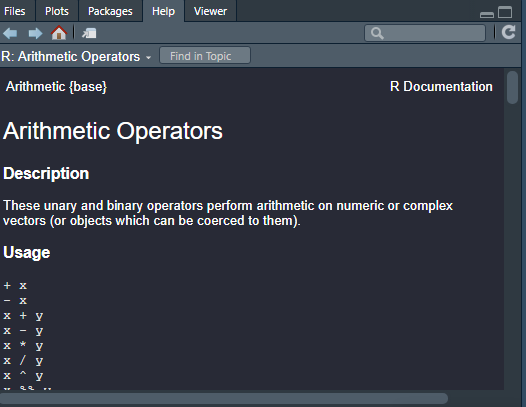
\includegraphics[width=1\linewidth]{images/aide}

Cette page décrit (en anglais) la fonction, ses arguments, son résultat, le tout accompagné de diverses notes, références et exemples. Ces pages d'aide contiennent à peu près tout ce que vous pourrez chercher à savoir, mais elles ne sont pas toujours d'une lecture aisée.

Un autre cas très courant dans R est de ne pas se souvenir ou de ne pas connaître le nom de la fonction effectuant une tâche donnée. Dans ce cas on se reportera aux différentes manières de trouver de l'aide décrites dans le chapitre Où trouver de l'aide ?.

\hypertarget{autocompluxe9tion}{%
\subsection{Autocomplétion}\label{autocompluxe9tion}}

RStudio fournit un outil bien pratique appelé autocomplétion. Saisissez les premières lettres d'une fonction, par exemple me puis appuyez sur la touche Tabulation. RStudio affichera la liste des fonctions dont le nom commence par me ainsi qu'un court descriptif de chacune. Un appui sur la touche Entrée provoquera la saisie du nom complet de la fonction choisie.

\hypertarget{premier-travail-avec-les-donnees}{%
\chapter{PREMIER TRAVAIL AVEC LES DONNEES}\label{premier-travail-avec-les-donnees}}

\hypertarget{regrouper-les-commandes-dans-des-scripts}{%
\section{Regrouper les commandes dans des scripts}\label{regrouper-les-commandes-dans-des-scripts}}

Jusqu'à maintenant nous avons utilisé uniquement la console pour communiquer avec R via l'invite de commandes. Le principal problème de ce mode d'interaction est qu'une fois qu'une commande est tapée, elle est pour ainsi dire « perdue », c'est-à-dire qu'on doit la saisir à nouveau si on veut l'exécuter une seconde fois. L'utilisation de la console est donc restreinte aux petites commandes « jetables », le plus souvent utilisées comme test.

La plupart du temps, les commandes seront stockées dans un fichier à part, que l'on pourra facilement ouvrir, éditer et exécuter en tout ou partie si besoin. On appelle en général ce type de fichier un script.

Pour comprendre comment cela fonctionne, dans RStudio cliquez sur l'icône en haut à gauche représentant un fichier avec un signe plus vert, puis choisissez R script.

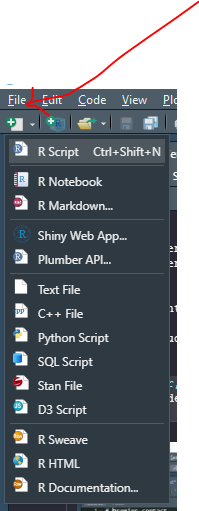
\includegraphics[width=1\linewidth]{images/script}

Un nouvel onglet apparaît dans le quadrant supérieur gauche.

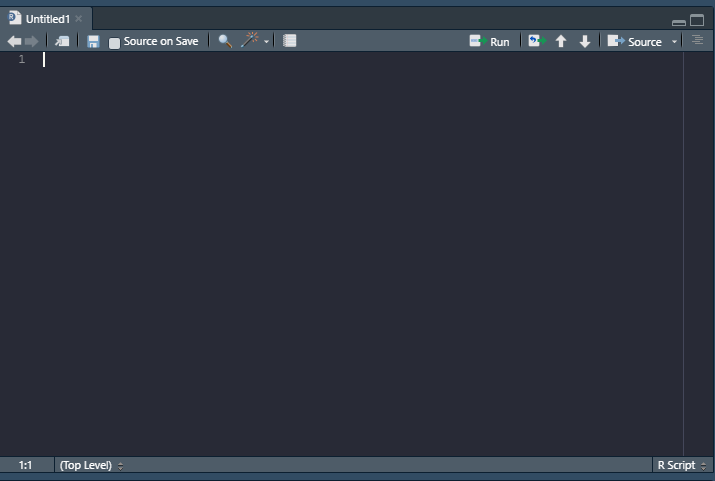
\includegraphics[width=1\linewidth]{images/espace_script}

Nous pouvons désormais y saisir des commandes. Par exemple, tapez sur la première ligne la commande suivante : 2 + 2. Ensuite, cliquez sur l'icône Run (en haut à droite de l'onglet du script) ou bien pressez simulatément les touches CTRL et Entrée.

Les lignes suivantes ont dû faire leur apparition dans la console :

\begin{Shaded}
\begin{Highlighting}[]
\DecValTok{2}\SpecialCharTok{+}\DecValTok{2}
\end{Highlighting}
\end{Shaded}

\begin{verbatim}
## [1] 4
\end{verbatim}

Voici donc comment soumettre rapidement à R les commandes saisies dans votre fichier. Vous pouvez désormais l'enregistrer, l'ouvrir plus tard, et en exécuter tout ou partie. À noter que vous avez plusieurs possibilités pour soumettre des commandes à R :

vous pouvez exécuter la ligne sur laquelle se trouve votre curseur en cliquant sur Run ou en pressant simulatément les touches CTRL et Entrée ; vous pouvez sélectionner plusieurs lignes contenant des commandes et les exécuter toutes en une seule fois exactement de la même manière ; vous pouvez exécuter d'un coup l'intégralité de votre fichier en cliquant sur l'icône Source. La plupart du travail sous R consistera donc à éditer un ou plusieurs fichiers de commandes et à envoyer régulièrement les commandes saisies à R en utilisant les raccourcis clavier ad hoc.

\hypertarget{ajouter-des-commentaires}{%
\subsection{Ajouter des commentaires}\label{ajouter-des-commentaires}}

Un commentaire est une ligne ou une portion de ligne qui sera ignorée par R. Ceci signifie qu'on peut y écrire ce qu'on veut et qu'on va les utiliser pour ajouter tout un tas de commentaires à notre code permettant de décrire les différentes étapes du travail, les choses à se rappeler, les questions en suspens, etc.

Un commentaire sous R commence par un ou plusieurs symboles \# (qui s'obtient avec les touches Alt Gr et 3 sur les claviers de type PC). Tout ce qui suit ce symbole jusqu'à la fin de la ligne est considéré comme un commentaire. On peut créer une ligne entière de commentaire en la faisant débuter par \#\#. Par exemple :

\begin{Shaded}
\begin{Highlighting}[]
\DocumentationTok{\#\# Tableau croisé de la CSP par le nombre de livres lus.}
\DocumentationTok{\#\# Attention au nombre de non réponses !}
\end{Highlighting}
\end{Shaded}

On peut aussi créer des commentaires pour une ligne en cours :

\begin{Shaded}
\begin{Highlighting}[]
\NormalTok{x }\OtherTok{\textless{}{-}} \DecValTok{2} \CommentTok{\# On met 2 dans x, parce qu\textquotesingle{}il le vaut bien}
\end{Highlighting}
\end{Shaded}

\textbf{NB}:\emph{Dans tous les cas, il est très important de documenter ses fichiers R au fur et à mesure, faute de quoi on risque de ne plus y comprendre grand chose si on les reprend ne serait-ce que quelques semaines plus tard.}

Avec RStudio, vous pouvez également utiliser les commentaires pour créer des sections au sein de votre script et naviguer plus rapidement. Il suffit de faire suivre une ligne de commentaires d'au moins 4 signes moins (----). Par exemple, si vous saisissez ceci dans votre script :

\begin{Shaded}
\begin{Highlighting}[]
\DocumentationTok{\#\# Créer les objets {-}{-}{-}{-}}

\NormalTok{x }\OtherTok{\textless{}{-}} \DecValTok{2}
\NormalTok{y }\OtherTok{\textless{}{-}} \DecValTok{5}

\DocumentationTok{\#\# Calculs {-}{-}{-}{-}}

\NormalTok{x }\SpecialCharTok{+}\NormalTok{ y}
\end{Highlighting}
\end{Shaded}

\begin{verbatim}
## [1] 7
\end{verbatim}

Vous verrez apparaître en bas à gauche de la fenêtre du script un symbole dièse orange. Si vous cliquez dessus, un menu de navigation s'affichera vous permettant de vous déplacez rapidement au sein de votre script.

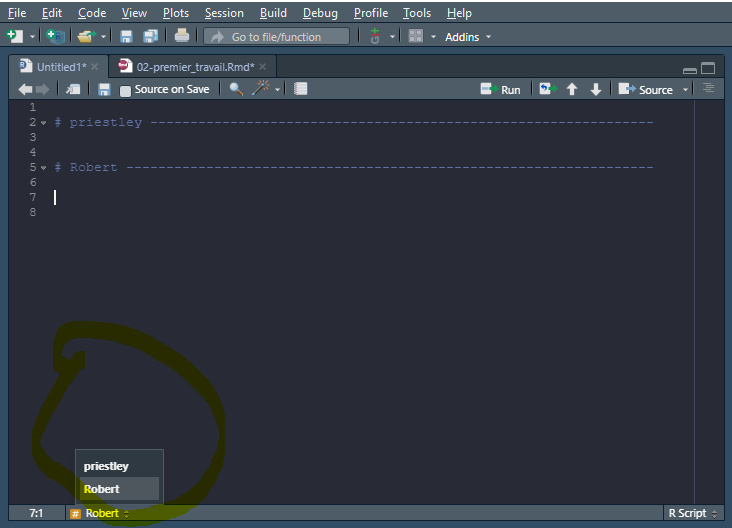
\includegraphics[width=1\linewidth]{images/script_section}

\textbf{Note} : on remarquera au passage que le titre de l'onglet est affiché en rouge et suivi d'une astérisque (*), nous indiquant ainsi qu'il y a des modifications non enregistrées dans notre
fichier

\hypertarget{tableaux-de-donnuxe9es}{%
\section{Tableaux de données}\label{tableaux-de-donnuxe9es}}

Dans cette partie nous allons utiliser un jeu de données inclus dans l'extension questionr. L'installation d'extension est décrite dans le chapitre Extensions.
Le jeu de données en question est un extrait de l'enquête Histoire de vie réalisée par l'INSEE en 2003. Il contient 2000 individus et 20 variables. Pour pouvoir utiliser ces données, il faut d'abord charger l'extension questionr (après l'avoir installée, bien entendu). Le chargement d'une extension en mémoire se fait à l'aide de la fonction library. Sous RStudio, vous pouvez également charger une extension en allant dans l'onglet Packages du quadrant inférieur droit qui liste l'ensemble des packages disponibles et en cliquant la case à cocher située à gauche du nom du package désiré.

\begin{Shaded}
\begin{Highlighting}[]
\FunctionTok{library}\NormalTok{(questionr)}
\end{Highlighting}
\end{Shaded}

Puis nous allons indiquer à R que nous souhaitons accéder au jeu de données hdv2003 à l'aide de la fonction data :

\begin{Shaded}
\begin{Highlighting}[]
  \FunctionTok{data}\NormalTok{(hdv2003)}
\end{Highlighting}
\end{Shaded}

Bien. Et maintenant, elles sont où mes données ? Et bien elles se trouvent dans un objet nommé hdv2003 désormais chargé en mémoire et accessible directement. D'ailleurs, cet objet est maintenant visible dans l'onglet Environment du quadrant supérieur droit.

Essayons de taper son nom à l'invite de commande :

\begin{Shaded}
\begin{Highlighting}[]
\NormalTok{hdv2003}
\end{Highlighting}
\end{Shaded}

Le résultat (non reproduit ici) ne ressemble pas forcément à grand-chose\ldots{} Il faut se rappeler que par défaut, lorsqu'on lui fournit seulement un nom d'objet, R essaye de l'afficher de la manière la meilleure (ou la moins pire) possible. La réponse à la commande hdv2003 n'est donc rien moins que l'affichage des données brutes contenues dans cet objet.

Ce qui signifie donc que l'intégralité de notre jeu de données est inclus dans l'objet nommé hdv2003 ! En effet, dans R, un objet peut très bien contenir un simple nombre, un vecteur ou bien le résultat d'une enquête tout entier. Dans ce cas, les objets sont appelés des data frames, ou tableaux de données. Ils peuvent être manipulés comme tout autre objet. Par exemple :

Résumons

Comme nous avons désormais décidé de saisir nos commandes dans un script et non plus directement dans la console, les premières lignes de notre fichier de travail sur les données de l'enquête Histoire de vie pourraient donc ressembler à ceci :

\begin{Shaded}
\begin{Highlighting}[]
\DocumentationTok{\#\# Chargement des extensions nécessaires {-}{-}{-}{-}}
\FunctionTok{library}\NormalTok{(questionr)}
\DocumentationTok{\#\# Jeu de données hdv2003 {-}{-}{-}{-}}
\FunctionTok{data}\NormalTok{(hdv2003)}
\NormalTok{d }\OtherTok{\textless{}{-}}\NormalTok{ hdv2003}
\end{Highlighting}
\end{Shaded}

\hypertarget{inspection-visuelle-des-donnuxe9es}{%
\subsection{Inspection visuelle des données}\label{inspection-visuelle-des-donnuxe9es}}

La particularité de R par rapport à d'autres logiciels comme \textbf{Modalisa ou SPSS} est de ne pas proposer, par défaut, de vue des données sous forme de tableau. Ceci peut parfois être un peu déstabilisant dans les premiers temps d'utilisation, même si l'on perd vite l'habitude et qu'on finit par se rendre compte que « voir » les données n'est pas forcément un gage de productivité ou de rigueur dans le traitement.

Néanmoins, R propose une interface permettant de visualiser le contenu d'un tableau de données à l'aide de la fonction \textbf{View} :

\begin{Shaded}
\begin{Highlighting}[]
\FunctionTok{View}\NormalTok{(d)}
\end{Highlighting}
\end{Shaded}

Sous RStudio, on peut aussi afficher la visionneusee (viewer) en cliquant sur la petite icône en forme de tableau située à droite de la ligne d'un tableau de données dans l'onglet Environment du quadrant supérieur droit (cf.~figure ci-après).

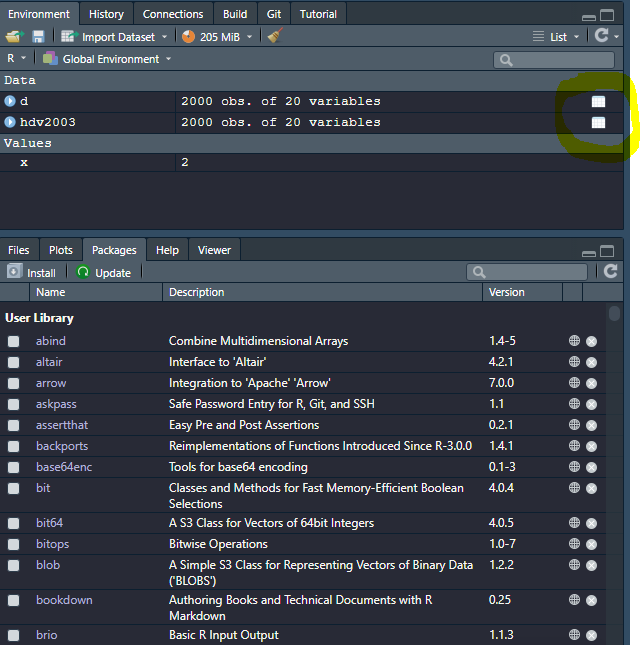
\includegraphics[width=1\linewidth]{images/visionneuse}
Dans tous les cas, RStudio lancera le viewer dans un onglet dédié dans le quadrant supérieur gauche. Le visualiseur de RStudio est plus avancé que celui-de base fournit par R. Il est possible de trier les données selon une variable en cliquant sur le nom de cette dernière. Il y a également un champs de recherche et un bouton Filter donnant accès à des options de filtrage avancées.

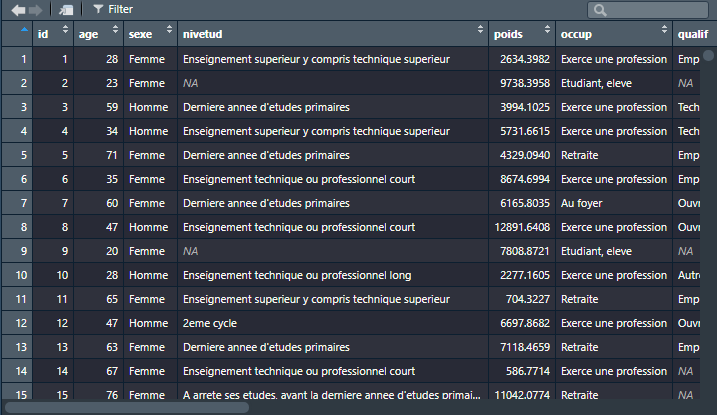
\includegraphics[width=1\linewidth]{images/viewer_pane}
\#\#\# Structure du tableau

Avant de travailler sur les données, nous allons essayer de comprendre comment elles sont structurées. Lors de l'import de données depuis un autre logiciel (que nous aborderons dans un autre chapitre), il s'agira souvent de vérifier que l'importation s'est bien déroulée.

Nous avons déjà vu qu'un tableau de données est organisé en lignes et en colonnes, les lignes correspondant aux observations et les colonnes aux variables. Les fonctions nrow, ncol et dim donnent respectivement le nombre de lignes, le nombre de colonnes et les dimensions de notre tableau. Nous pouvons donc d'ores et déjà vérifier que nnombre des lignes

\begin{Shaded}
\begin{Highlighting}[]
\FunctionTok{nrow}\NormalTok{(d)}\CommentTok{\#Nombre de lignes:}
\end{Highlighting}
\end{Shaded}

\begin{verbatim}
## [1] 2000
\end{verbatim}

\begin{Shaded}
\begin{Highlighting}[]
\FunctionTok{ncol}\NormalTok{(d)}\CommentTok{\#nombre de colonnes :}
\end{Highlighting}
\end{Shaded}

\begin{verbatim}
## [1] 20
\end{verbatim}

\begin{Shaded}
\begin{Highlighting}[]
\FunctionTok{dim}\NormalTok{(d)}\CommentTok{\# lignes x colonnes}
\end{Highlighting}
\end{Shaded}

\begin{verbatim}
## [1] 2000   20
\end{verbatim}

La fonction \textbf{names} donne les noms des colonnes de notre tableau, c'est-à-dire les noms des variables :

\begin{Shaded}
\begin{Highlighting}[]
\FunctionTok{names}\NormalTok{(d)}
\end{Highlighting}
\end{Shaded}

\begin{verbatim}
##  [1] "id"            "age"           "sexe"          "nivetud"      
##  [5] "poids"         "occup"         "qualif"        "freres.soeurs"
##  [9] "clso"          "relig"         "trav.imp"      "trav.satisf"  
## [13] "hard.rock"     "lecture.bd"    "peche.chasse"  "cuisine"      
## [17] "bricol"        "cinema"        "sport"         "heures.tv"
\end{verbatim}

\hypertarget{accuxe9der-aux-variables}{%
\subsection{Accéder aux variables}\label{accuxe9der-aux-variables}}

d représente donc l'ensemble de notre tableau de données. Nous avons vu que si l'on saisit simplement d à l'invite de commandes, on obtient un affichage du tableau en question. Mais comment accéder aux variables, c'est à dire aux colonnes de notre tableau ?
La réponse est simple : on utilise le nom de l'objet, suivi de l'opérateur \$, suivi du nom de la variable, comme ceci :

\begin{Shaded}
\begin{Highlighting}[]
\NormalTok{d}\SpecialCharTok{$}\NormalTok{sexe}
\end{Highlighting}
\end{Shaded}

Au regard du résultat (non reproduit ici), on constate alors que R a bien accédé au contenu de notre variable sexe du tableau d et a affiché son contenu, c'est-à-dire l'ensemble des valeurs prises par la variable.

Les fonctions head et tail permettent d'afficher seulement les premières (respectivement les dernières) valeurs prises par la variable. On peut leur passer en argument le nombre d'éléments à afficher :

\begin{Shaded}
\begin{Highlighting}[]
\FunctionTok{head}\NormalTok{(d}\SpecialCharTok{$}\NormalTok{nivetud)}\CommentTok{\# 6 premierès observations}
\end{Highlighting}
\end{Shaded}

\begin{verbatim}
## [1] Enseignement superieur y compris technique superieur
## [2] <NA>                                                
## [3] Derniere annee d'etudes primaires                   
## [4] Enseignement superieur y compris technique superieur
## [5] Derniere annee d'etudes primaires                   
## [6] Enseignement technique ou professionnel court       
## 8 Levels: N'a jamais fait d'etudes ...
\end{verbatim}

\begin{Shaded}
\begin{Highlighting}[]
\FunctionTok{tail}\NormalTok{(d}\SpecialCharTok{$}\NormalTok{age, }\DecValTok{10}\NormalTok{)}\CommentTok{\#10 dernières observations }
\end{Highlighting}
\end{Shaded}

\begin{verbatim}
##  [1] 52 42 50 41 46 45 46 24 24 66
\end{verbatim}

À noter que ces fonctions marchent aussi pour afficher les lignes du tableau d :

\begin{Shaded}
\begin{Highlighting}[]
\FunctionTok{head}\NormalTok{(d,}\DecValTok{2}\NormalTok{)}
\end{Highlighting}
\end{Shaded}

\begin{verbatim}
##   id age  sexe                                              nivetud    poids
## 1  1  28 Femme Enseignement superieur y compris technique superieur 2634.398
## 2  2  23 Femme                                                 <NA> 9738.396
##                   occup  qualif freres.soeurs clso                       relig
## 1 Exerce une profession Employe             8  Oui Ni croyance ni appartenance
## 2       Etudiant, eleve    <NA>             2  Oui Ni croyance ni appartenance
##        trav.imp    trav.satisf hard.rock lecture.bd peche.chasse cuisine bricol
## 1 Peu important Insatisfaction       Non        Non          Non     Oui    Non
## 2          <NA>           <NA>       Non        Non          Non     Non    Non
##   cinema sport heures.tv
## 1    Non   Non         0
## 2    Oui   Oui         1
\end{verbatim}

\hypertarget{la-fonction-str}{%
\subsection{\texorpdfstring{La fonction \textbf{str}}{La fonction str}}\label{la-fonction-str}}

La fonction str est plus complète que names. Elle liste les différentes variables, indique leur type et donne le cas échéant des informations supplémentaires ainsi qu'un échantillon des premières valeurs prises par cette variable :

\begin{Shaded}
\begin{Highlighting}[]
\FunctionTok{str}\NormalTok{(d)}
\end{Highlighting}
\end{Shaded}

\begin{verbatim}
## 'data.frame':    2000 obs. of  20 variables:
##  $ id           : int  1 2 3 4 5 6 7 8 9 10 ...
##  $ age          : int  28 23 59 34 71 35 60 47 20 28 ...
##  $ sexe         : Factor w/ 2 levels "Homme","Femme": 2 2 1 1 2 2 2 1 2 1 ...
##  $ nivetud      : Factor w/ 8 levels "N'a jamais fait d'etudes",..: 8 NA 3 8 3 6 3 6 NA 7 ...
##  $ poids        : num  2634 9738 3994 5732 4329 ...
##  $ occup        : Factor w/ 7 levels "Exerce une profession",..: 1 3 1 1 4 1 6 1 3 1 ...
##  $ qualif       : Factor w/ 7 levels "Ouvrier specialise",..: 6 NA 3 3 6 6 2 2 NA 7 ...
##  $ freres.soeurs: int  8 2 2 1 0 5 1 5 4 2 ...
##  $ clso         : Factor w/ 3 levels "Oui","Non","Ne sait pas": 1 1 2 2 1 2 1 2 1 2 ...
##  $ relig        : Factor w/ 6 levels "Pratiquant regulier",..: 4 4 4 3 1 4 3 4 3 2 ...
##  $ trav.imp     : Factor w/ 4 levels "Le plus important",..: 4 NA 2 3 NA 1 NA 4 NA 3 ...
##  $ trav.satisf  : Factor w/ 3 levels "Satisfaction",..: 2 NA 3 1 NA 3 NA 2 NA 1 ...
##  $ hard.rock    : Factor w/ 2 levels "Non","Oui": 1 1 1 1 1 1 1 1 1 1 ...
##  $ lecture.bd   : Factor w/ 2 levels "Non","Oui": 1 1 1 1 1 1 1 1 1 1 ...
##  $ peche.chasse : Factor w/ 2 levels "Non","Oui": 1 1 1 1 1 1 2 2 1 1 ...
##  $ cuisine      : Factor w/ 2 levels "Non","Oui": 2 1 1 2 1 1 2 2 1 1 ...
##  $ bricol       : Factor w/ 2 levels "Non","Oui": 1 1 1 2 1 1 1 2 1 1 ...
##  $ cinema       : Factor w/ 2 levels "Non","Oui": 1 2 1 2 1 2 1 1 2 2 ...
##  $ sport        : Factor w/ 2 levels "Non","Oui": 1 2 2 2 1 2 1 1 1 2 ...
##  $ heures.tv    : num  0 1 0 2 3 2 2.9 1 2 2 ...
\end{verbatim}

La première ligne nous informe qu'il s'agit bien d'un tableau de données avec 2000 observations et 20 variables. Vient ensuite la liste des variables. La première se nomme id et est de type entier (int). La seconde se nomme age et est de type numérique. La troisième se nomme sexe, il s'agit d'un facteur (factor).

Un facteur est une variable pouvant prendre un nombre limité de modalités (levels). Ici notre variable a deux modalités possibles : « Homme » et « Femme ». Ce type de variable est décrit plus en détail dans le chapitre sur la manipulation de données.

\textbf{Important}

La fonction str est essentielle à connaître et peut s'appliquer à n'importe quel type d'objet. C'est un excellent moyen de connaître en détail la structure d'un objet. Cependant, les résultats peuvent être parfois trop détaillés et on lui priviligiera dans certains cas la fonction describe que l'on abordera dans les prochains chapitres, cependant moins générique puisque ne s'appliquant qu'à des tableaux de données et à des vecteurs, tandis que str peut s'appliquer à absolument tout objet, y compris des fonctions.

\begin{Shaded}
\begin{Highlighting}[]
\FunctionTok{describe}\NormalTok{(d)}
\end{Highlighting}
\end{Shaded}

\begin{verbatim}
## [2000 obs. x 20 variables] tbl_df tbl data.frame
## 
## $id: 
## integer: 1 2 3 4 5 6 7 8 9 10 ...
## min: 1 - max: 2000 - NAs: 0 (0%) - 2000 unique values
## 
## $age: 
## integer: 28 23 59 34 71 35 60 47 20 28 ...
## min: 18 - max: 97 - NAs: 0 (0%) - 78 unique values
## 
## $sexe: 
## nominal factor: "Femme" "Femme" "Homme" "Homme" "Femme" "Femme" "Femme" "Homme" "Femme" "Homme" ...
## 2 levels: Homme | Femme
## NAs: 0 (0%)
## 
## $nivetud: 
## nominal factor: "Enseignement superieur y compris technique superieur" NA "Derniere annee d'etudes primaires" "Enseignement superieur y compris technique superieur" "Derniere annee d'etudes primaires" "Enseignement technique ou professionnel court" "Derniere annee d'etudes primaires" "Enseignement technique ou professionnel court" NA "Enseignement technique ou professionnel long" ...
## 8 levels: N'a jamais fait d'etudes | A arrete ses etudes, avant la derniere annee d'etudes primaires | Derniere annee d'etudes primaires | 1er cycle | 2eme cycle | Enseignement technique ou professionnel court | Enseignement technique ou professionnel long | Enseignement superieur y compris technique superieur
## NAs: 112 (5.6%)
## 
## $poids: 
## numeric: 2634.3982157 9738.3957759 3994.1024587 5731.6615081 4329.0940022 8674.6993828 6165.8034861 12891.640759 7808.8720636 2277.160471 ...
## min: 78.0783403 - max: 31092.14132 - NAs: 0 (0%) - 1877 unique values
## 
## $occup: 
## nominal factor: "Exerce une profession" "Etudiant, eleve" "Exerce une profession" "Exerce une profession" "Retraite" "Exerce une profession" "Au foyer" "Exerce une profession" "Etudiant, eleve" "Exerce une profession" ...
## 7 levels: Exerce une profession | Chomeur | Etudiant, eleve | Retraite | Retire des affaires | Au foyer | Autre inactif
## NAs: 0 (0%)
## 
## $qualif: 
## nominal factor: "Employe" NA "Technicien" "Technicien" "Employe" "Employe" "Ouvrier qualifie" "Ouvrier qualifie" NA "Autre" ...
## 7 levels: Ouvrier specialise | Ouvrier qualifie | Technicien | Profession intermediaire | Cadre | Employe | Autre
## NAs: 347 (17.3%)
## 
## $freres.soeurs: 
## integer: 8 2 2 1 0 5 1 5 4 2 ...
## min: 0 - max: 22 - NAs: 0 (0%) - 19 unique values
## 
## $clso: 
## nominal factor: "Oui" "Oui" "Non" "Non" "Oui" "Non" "Oui" "Non" "Oui" "Non" ...
## 3 levels: Oui | Non | Ne sait pas
## NAs: 0 (0%)
## 
## $relig: 
## nominal factor: "Ni croyance ni appartenance" "Ni croyance ni appartenance" "Ni croyance ni appartenance" "Appartenance sans pratique" "Pratiquant regulier" "Ni croyance ni appartenance" "Appartenance sans pratique" "Ni croyance ni appartenance" "Appartenance sans pratique" "Pratiquant occasionnel" ...
## 6 levels: Pratiquant regulier | Pratiquant occasionnel | Appartenance sans pratique | Ni croyance ni appartenance | Rejet | NSP ou NVPR
## NAs: 0 (0%)
## 
## $trav.imp: 
## nominal factor: "Peu important" NA "Aussi important que le reste" "Moins important que le reste" NA "Le plus important" NA "Peu important" NA "Moins important que le reste" ...
## 4 levels: Le plus important | Aussi important que le reste | Moins important que le reste | Peu important
## NAs: 952 (47.6%)
## 
## $trav.satisf: 
## nominal factor: "Insatisfaction" NA "Equilibre" "Satisfaction" NA "Equilibre" NA "Insatisfaction" NA "Satisfaction" ...
## 3 levels: Satisfaction | Insatisfaction | Equilibre
## NAs: 952 (47.6%)
## 
## $hard.rock: 
## nominal factor: "Non" "Non" "Non" "Non" "Non" "Non" "Non" "Non" "Non" "Non" ...
## 2 levels: Non | Oui
## NAs: 0 (0%)
## 
## $lecture.bd: 
## nominal factor: "Non" "Non" "Non" "Non" "Non" "Non" "Non" "Non" "Non" "Non" ...
## 2 levels: Non | Oui
## NAs: 0 (0%)
## 
## $peche.chasse: 
## nominal factor: "Non" "Non" "Non" "Non" "Non" "Non" "Oui" "Oui" "Non" "Non" ...
## 2 levels: Non | Oui
## NAs: 0 (0%)
## 
## $cuisine: 
## nominal factor: "Oui" "Non" "Non" "Oui" "Non" "Non" "Oui" "Oui" "Non" "Non" ...
## 2 levels: Non | Oui
## NAs: 0 (0%)
## 
## $bricol: 
## nominal factor: "Non" "Non" "Non" "Oui" "Non" "Non" "Non" "Oui" "Non" "Non" ...
## 2 levels: Non | Oui
## NAs: 0 (0%)
## 
## $cinema: 
## nominal factor: "Non" "Oui" "Non" "Oui" "Non" "Oui" "Non" "Non" "Oui" "Oui" ...
## 2 levels: Non | Oui
## NAs: 0 (0%)
## 
## $sport: 
## nominal factor: "Non" "Oui" "Oui" "Oui" "Non" "Oui" "Non" "Non" "Non" "Oui" ...
## 2 levels: Non | Oui
## NAs: 0 (0%)
## 
## $heures.tv: 
## numeric: 0 1 0 2 3 2 2.9 1 2 2 ...
## min: 0 - max: 12 - NAs: 5 (0.2%) - 30 unique values
\end{verbatim}

\hypertarget{quelques-calculs-simples}{%
\subsection{Quelques calculs simples}\label{quelques-calculs-simples}}

Maintenant que nous savons accéder aux variables, effectuons quelques calculs simples comme la moyenne, la médiane, le minimum et le maximum, à l'aide des fonctions mean, median, min et max.

\begin{Shaded}
\begin{Highlighting}[]
\FunctionTok{mean}\NormalTok{(d}\SpecialCharTok{$}\NormalTok{age)}
\end{Highlighting}
\end{Shaded}

\begin{verbatim}
## [1] 48.157
\end{verbatim}

\begin{Shaded}
\begin{Highlighting}[]
\FunctionTok{median}\NormalTok{(d}\SpecialCharTok{$}\NormalTok{age)}
\end{Highlighting}
\end{Shaded}

\begin{verbatim}
## [1] 48
\end{verbatim}

\begin{Shaded}
\begin{Highlighting}[]
\FunctionTok{min}\NormalTok{(d}\SpecialCharTok{$}\NormalTok{age)}
\end{Highlighting}
\end{Shaded}

\begin{verbatim}
## [1] 18
\end{verbatim}

\begin{Shaded}
\begin{Highlighting}[]
\FunctionTok{max}\NormalTok{(d}\SpecialCharTok{$}\NormalTok{age)}
\end{Highlighting}
\end{Shaded}

\begin{verbatim}
## [1] 97
\end{verbatim}

\begin{blackbox}

\begin{center}
\textbf{Attention!}

\end{center}

Au sens strict, il ne s'agit pas d'un véritable âge moyen puisqu'il faudrait ajouter 0,5 à cette valeur calculée, un âge moyen se calculant à partir d'âges exacts et non à partir âges révolus.

\end{blackbox}

On peut aussi très facilement obtenir un tri à plat à l'aide la fonction \textbf{table}

\begin{Shaded}
\begin{Highlighting}[]
\FunctionTok{table}\NormalTok{(d}\SpecialCharTok{$}\NormalTok{qualif)}
\end{Highlighting}
\end{Shaded}

\begin{verbatim}
## 
##       Ouvrier specialise         Ouvrier qualifie               Technicien 
##                      203                      292                       86 
## Profession intermediaire                    Cadre                  Employe 
##                      160                      260                      594 
##                    Autre 
##                       58
\end{verbatim}

La fonction \textbf{summary}, bien pratique, permet d'avoir une vue résumée d'une variable. Elle s'applique à tout type d'objets (y compris un tableau de données entier) et s'adapte à celui-ci.

\begin{Shaded}
\begin{Highlighting}[]
\FunctionTok{summary}\NormalTok{(d}\SpecialCharTok{$}\NormalTok{age)}
\end{Highlighting}
\end{Shaded}

\begin{verbatim}
##    Min. 1st Qu.  Median    Mean 3rd Qu.    Max. 
##   18.00   35.00   48.00   48.16   60.00   97.00
\end{verbatim}

\begin{Shaded}
\begin{Highlighting}[]
\FunctionTok{summary}\NormalTok{(d}\SpecialCharTok{$}\NormalTok{qualif)}
\end{Highlighting}
\end{Shaded}

\begin{verbatim}
##       Ouvrier specialise         Ouvrier qualifie               Technicien 
##                      203                      292                       86 
## Profession intermediaire                    Cadre                  Employe 
##                      160                      260                      594 
##                    Autre                     NA's 
##                       58                      347
\end{verbatim}

\hypertarget{nos-premiers-graphiques}{%
\section{Nos premiers graphiques}\label{nos-premiers-graphiques}}

R est très puissant en termes de représentations graphiques, notamment grâce à des extensions dédiées. Pour l'heure contentons-nous d'un premier essai à l'aide de la fonction générique \href{http://rdrr.io/pkg/graphics/sym/plot}{plot}.

\begin{Shaded}
\begin{Highlighting}[]
\FunctionTok{plot}\NormalTok{(d}\SpecialCharTok{$}\NormalTok{hard.rock,d}\SpecialCharTok{$}\NormalTok{age)}
\end{Highlighting}
\end{Shaded}

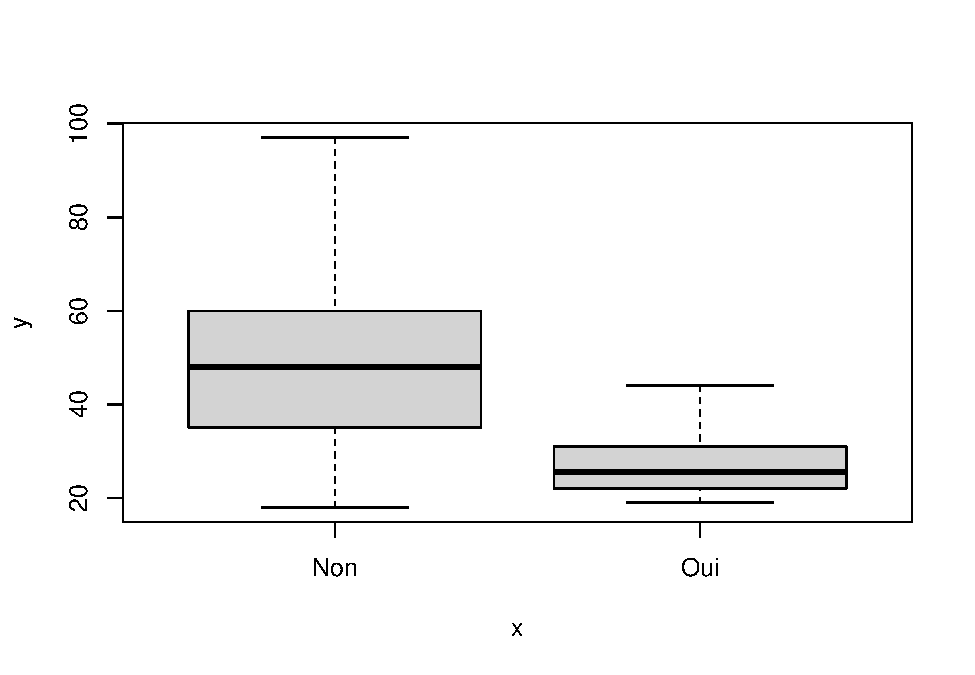
\includegraphics{bookdownproj_files/figure-latex/unnamed-chunk-65-1.pdf}
Il semblerait bien que les amateurs de hard rock soient plus jeunes.
Nous n'avons qu'entr'aperçu les possibilités de R. Avant de pouvoir nous lancer dans des analyses statisques, il est préférable de revenir un peu aux fondamentaux de R (les types d'objets, la syntaxe, le recodage de variables\ldots) mais aussi comment installer des extensions, importer des données, etc. Nous vous conseillons donc de poursuivre la lecture de la section Prise en main puis de vous lancer à l'assault de la section Statistique introductive.

\hypertarget{extensions-installation-mise-uxe0-jour}{%
\chapter{Extensions (installation, mise à jour)}\label{extensions-installation-mise-uxe0-jour}}

\hypertarget{pruxe9sentation}{%
\section{Présentation}\label{pruxe9sentation}}

L'installation par défaut du logiciel R contient le cœur du programme ainsi qu'un ensemble de fonctions de base fournissant un grand nombre d'outils de traitement de données et d'analyse statistiques.

R étant un logiciel libre, il bénéficie d'une forte communauté d'utilisateurs qui peuvent librement contribuer au développement du logiciel en lui ajoutant des fonctionnalités supplémentaires. Ces contributions prennent la forme d'extensions (packages en anglais) pouvant être installées par l'utilisateur et fournissant alors diverses fonctionnalités supplémentaires.

Il existe un très grand nombre d'extensions (plus de 6500 à ce jour), qui sont diffusées par un réseau baptisé CRAN (Comprehensive R Archive Network).

La liste de toutes les extensions disponibles sur CRAN est disponible ici:\href{https://cran.r-project.org/web/packages/available_packages_by_date.html}{tous les packages}

Pour faciliter un peu le repérage des extensions, il existe un ensemble de regroupements thématiques (économétrie, finance, génétique, données spatiales\ldots) baptisés Task views :
\href{http://cran.r-project.org/web/views/}{recherche des packages par thème}
On y trouve notamment une Task view dédiée aux sciences sociales, listant de nombreuses extensions potentiellement utiles pour les analyses statistiques dans ce champ disciplinaire :
\href{http://cran.r-project.org/web/views/SocialSciences.html.}{Packages pour les analyses statistiques avec les sciences sociales}
On peut aussi citer le site Awesome R\url{https://github.com/qinwf/awesome-R}:qui fournit une liste d'extensions choisies et triées par thématique.

\hypertarget{le-tidyverse}{%
\section{Le tidyverse}\label{le-tidyverse}}

Hadley Wickham est professeur associé à l'université de Rice et scientifique en chef à Rstudio. Il a développé de nombreux extensions pour R (plus d'une cinquantaine à ce jours) qui, pour la plupart, fonctionne de manière harmonisée entre elles. Par ailleurs, la plupart s'intègre parfaitement avec RStudio.

Pour certaines tâches, il peut exister plusieurs solutions / extensions différentes pour les réaliser. Dans la mesure où il n'est pas possible d'être exhaustif, nous avons fait le choix dans le cadre de cette initiation de choisir en priorité, lorsque cela est possible, les extensions du tidyverse, en particulier \href{http://rdrr.io/pkg/haven}{haven}, \href{http://rdrr.io/pkg/readr}{readr} et \href{http://rdrr.io/pkg/readxl}{readxl} pour l'import de données, \href{http://rdrr.io/pkg/dplyr}{dplyr}, \href{http://rdrr.io/pkg/dplyr}{tidyr} ou reshape2 pour la manipulation de données, \href{}{ggplot2} pour les graphiques, \href{http://rdrr.io/pkg/lubridate}{lubridate} pour la gestion des dates, \href{http://rdrr.io/pkg/forcats}{forcats} pour la manipulation des facteurs ou encore \href{http://rdrr.io/pkg/stringr}{stringr} pour la manipulation de chaînes de caractères.

Il existe par ailleurs une extension homonyme \href{http://rdrr.io/pkg/tidyverse}{tidyverse}. L'installation (voir ci-dessous) de cette extension permets l'installation automatique de l'ensemble des autres extensions du tidyverse. Le chargement de cette extension avec la fonction library (voir ci-après) permets de charger en mémoire en une seule opération les principales extensions du tidyverse, à savoir \href{(http://rdrr.io/pkg/ggplot2)}{ggplot2}, \href{http://rdrr.io/pkg/tibble}{tibble}, \href{http://rdrr.io/pkg/tidyr}{tidyr}, \href{http://rdrr.io/pkg/readr}{readr}, \href{http://rdrr.io/pkg/purrr}{purrr} et \href{http://rdrr.io/pkg/dplyr}{dplyr}.

Nous allons passer au peigne-fin certains packages du \href{http://rdrr.io/pkg/tidyverse}{tidyverse}.

\hypertarget{installation-depuis-cran}{%
\section{Installation depuis CRAN}\label{installation-depuis-cran}}

L'installation d'une extension se fait par la fonction \href{http://rdrr.io/pkg/utils/sym/install.packages}{install.packages}, à qui on fournit le nom de l'extension. Par exemple, si on souhaite installer l'extension ade4 :

\begin{Shaded}
\begin{Highlighting}[]
\FunctionTok{install.packages}\NormalTok{(}\StringTok{"classlnt"}\NormalTok{, }\AttributeTok{dep =} \ConstantTok{TRUE}\NormalTok{)}
\end{Highlighting}
\end{Shaded}

L'option dep=TRUE indique à R de télécharger et d'installer également toutes les extensions dont l'extension choisie dépend pour son fonctionnement.

Sous RStudio, on pourra également cliquer sur Install dans l'onglet Packages du quadrant inférieur droit comme l'indique cette image :

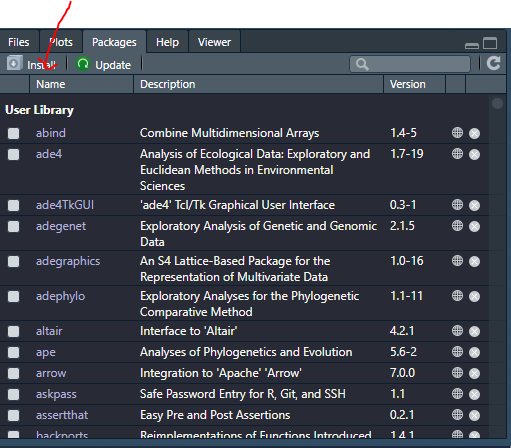
\includegraphics[width=0.7\linewidth]{images/packages}
Une fois l'extension installée, elle peut être appelée depuis la console ou un fichier script avec la fonction library ou la fonction require :

\begin{Shaded}
\begin{Highlighting}[]
\FunctionTok{library}\NormalTok{(ade4)}
\end{Highlighting}
\end{Shaded}

ou

\begin{Shaded}
\begin{Highlighting}[]
\FunctionTok{require}\NormalTok{(ade4)}
\end{Highlighting}
\end{Shaded}

À partir de là, on peut utiliser les fonctions de l'extension, consulter leur page d'aide en ligne, accéder aux jeux de données qu'elle contient, etc.

Pour mettre à jour l'ensemble des extensions installées, \textless dfndata-index=``mise à jour, extensions''\textgreater{} la fonction \href{http://rdrr.io/pkg/utils/sym/update.packages}{update.packages} suffit :

\begin{Shaded}
\begin{Highlighting}[]
\FunctionTok{update.packages}\NormalTok{(}\StringTok{"ade4"}\NormalTok{)}
\end{Highlighting}
\end{Shaded}

ou
Sous RStudio, on pourra alternativement cliquer sur Update dans l'onglet Packages du quadrant inférieur droit.

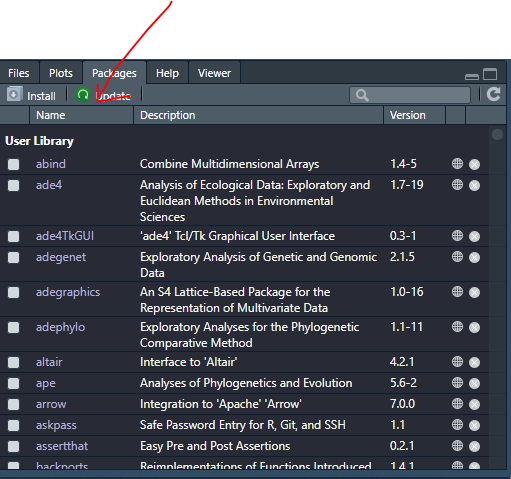
\includegraphics[width=0.75\linewidth]{images/packages2}
Si on souhaite désinstaller une extension précédemment installée, on peut utiliser la fonction \href{http://rdrr.io/pkg/utils/sym/remove.packages}{remove.packages} :

\begin{Shaded}
\begin{Highlighting}[]
\FunctionTok{remove.packages}\NormalTok{(}\StringTok{"classlnt"}\NormalTok{)}
\end{Highlighting}
\end{Shaded}

\begin{redbox}

\begin{center}
\textbf{Important!}

\end{center}

Il est important de bien comprendre la différence entre \href{http://rdrr.io/pkg/utils/sym/install.packages}{install.packages} et \href{http://rdrr.io/pkg/utils/sym/install.packages}{library}. La première va chercher les extensions sur internet et les installe en local sur le disque dur de l'ordinateur. On n'a besoin d'effectuer cette opération qu'une seule fois. La seconde lit les informations de l'extension sur le disque dur et les met à disposition de R. On a besoin de l'exécuter à chaque début de session ou de script.

\end{redbox}

\hypertarget{installation-depuis-github}{%
\section{Installation depuis GitHub}\label{installation-depuis-github}}

Certains \href{https://github.com/}{packages} sont développés sur GitHub. Dès lors, la version de développement sur GitHub peut contenir des fonctions qui ne sont pas encore disponibles dans la version stable disponible sur CRAN. Ils arrivent aussi parfois que certains packages ne soient disponibles que sur GitHub.
L'installation d'un package depuis GitHub est très facile grâce à la fonction \href{http://rdrr.io/pkg/devtools/sym/install_github}{install\_github} de l'extension \href{http://rdrr.io/pkg/devtools}{devtools} (que l'on aura préalablement installée depuis CRAN ;-) )

\hypertarget{introduction-au-tidyverse}{%
\chapter{Introduction au tidyverse}\label{introduction-au-tidyverse}}

\hypertarget{extensions}{%
\section{Extensions}\label{extensions}}

Le terme tidyverse est une contraction de tidy (qu'on pourrait traduire par ``bien rangé'') et de universe. Il s'agit en fait d'une collection d'extensions conçues pour travailler ensemble et basées sur une philosophie commune.

Elles abordent un très grand nombre d'opérations courantes dans R (la liste n'est pas exhaustive) :
- visualisation
- manipulation des tableaux de données
- import/export de données
- manipulation de variables
- extraction de données du Web
- programmation

Un des objectifs de ces extensions est de fournir des fonctions avec une syntaxe cohérente, qui fonctionnent bien ensemble, et qui retournent des résultats prévisibles. Elles sont en grande partie issues du travail \href{http://hadley.nz/}{d'Hadley Wickham}, qui travaille désormais pour \href{https://www.rstudio.com/}{RStudio}
\#\# Installation

\begin{Shaded}
\begin{Highlighting}[]
\FunctionTok{install.packages}\NormalTok{(}\StringTok{"tidyverse"}\NormalTok{)}
\end{Highlighting}
\end{Shaded}

Cette commande va en fait installer plusieurs extensions qui constituent le coeur du tidyverse, à savoir :
- \href{http://rdrr.io/pkg/ggplot2}{ggplot2} (visualisation)
- \href{http://rdrr.io/pkg/dplyr}{dplyr} (manipulation des données)
- \href{http://rdrr.io/pkg/tidyr}{tidyr} (remise en forme des données)
- \href{http://rdrr.io/pkg/purrr}{purrr} (programmation)
- \href{http://rdrr.io/pkg/readr}{readr} (importation de données)
- \href{http://rdrr.io/pkg/tibble}{tibble} (tableaux de données)
- \href{http://rdrr.io/pkg/forcats}{forcats} (variables qualitatives)
- \href{http://rdrr.io/pkg/stringr}{stringr} (chaînes de caractères)
De la même manière, charger l'extension avec :

\begin{Shaded}
\begin{Highlighting}[]
\FunctionTok{library}\NormalTok{(tidyverse)}
\end{Highlighting}
\end{Shaded}

Chargera l'ensemble des extensions précédentes.

Il existe d'autres extensions qui font partie du \href{http://rdrr.io/pkg/tidyverse}{tidyverse} mais qui doivent être chargées explicitement, comme par exemple \href{http://rdrr.io/pkg/readxl}{readxl} (pour l'importation de données depuis des fichiers Excel).

La liste complète des extensions se trouve sur \href{https://www.tidyverse.org/packages/}{le site officiel du tidyverse}

\hypertarget{tidy-data}{%
\section{tidy data}\label{tidy-data}}

Le \href{http://rdrr.io/pkg/tidyverse}{tidyverse} est en partie fondé sur le concept de tidy data, développé à l'origine par Hadley Wickham dans \href{https://www.jstatsoft.org/article/view/v059i10}{un article de 2014}du Journal of Statistical Software.
Il s'agit d'un modèle d'organisation des données qui vise à faciliter le travail souvent long et fastidieux de nettoyage et de préparation préalable à la mise en oeuvre de méthodes d'analyse.

Les principes d'un jeu de données tidy sont les suivants :

\begin{enumerate}
\def\labelenumi{\arabic{enumi}.}
\tightlist
\item
  chaque variable est une colonne
\item
  chaque observation est une ligne
\item
  chaque type d'observation est dans une table différente
\end{enumerate}

Un chapitre entier sera dédié à tidyr comment définir et rendre des données tidy avec l'extension tidyr.

Les extensions du \href{http://rdrr.io/pkg/tidyverse}{tidyverse}, notamment \href{http://rdrr.io/pkg/ggplot2}{ggplot2} et \href{http://rdrr.io/pkg/dplyr}{dplyr}, sont prévues pour fonctionner avec des données tidy

\hypertarget{tibbles}{%
\section{tibbles}\label{tibbles}}

Une autre particularité du tidyverse est que ces extensions travaillent avec des tableaux de données au format \href{http://rdrr.io/pkg/tibble/sym/tibble}{tibble}, qui est une évolution plus moderne du classique data frame du R de base. Ce format est fourni est géré par l'extension du même nom \href{http://rdrr.io/pkg/tibble/sym/tibble}{(tibble)}, qui fait partie du coeur du tidyverse. La plupart des fonctions des extensions du tidyverse acceptent des data frames en entrée, mais retournent un objet de classe tibble.

Contrairement aux data frames, les tibbles :

\begin{itemize}
\tightlist
\item
  n'ont pas de noms de lignes (rownames)
\item
  autorisent des noms de colonnes invalides pour les data frames (espaces, caractères spéciaux, nombres\ldots)
\item
  s'affichent plus intelligemment que les data frames : seules les premières lignes sont affichées, ainsi que quelques informations supplémentaires utiles (dimensions, types des colonnes\ldots)
\item
  ne font pas de partial matching sur les noms de colonnes
\item
  affichent un avertissement si on essaie d'accéder à une colonne qui n'existe pas
  Pour autant, les tibbles restent compatibles avec les data frames. On peut ainsi facilement convertir un data frame en tibble avec as\_tibble :
\end{itemize}

\begin{Shaded}
\begin{Highlighting}[]
\NormalTok{d }\OtherTok{\textless{}{-}} \FunctionTok{as.tibble}\NormalTok{(}\FunctionTok{rownames\_to\_column}\NormalTok{(mtcars))}
\end{Highlighting}
\end{Shaded}

\begin{verbatim}
## Warning: `as.tibble()` was deprecated in tibble 2.0.0.
## Please use `as_tibble()` instead.
## The signature and semantics have changed, see `?as_tibble`.
## This warning is displayed once every 8 hours.
## Call `lifecycle::last_lifecycle_warnings()` to see where this warning was generated.
\end{verbatim}

\begin{Shaded}
\begin{Highlighting}[]
\NormalTok{d}
\end{Highlighting}
\end{Shaded}

\begin{verbatim}
## # A tibble: 32 x 12
##    rowname       mpg   cyl  disp    hp  drat    wt  qsec    vs    am  gear  carb
##    <chr>       <dbl> <dbl> <dbl> <dbl> <dbl> <dbl> <dbl> <dbl> <dbl> <dbl> <dbl>
##  1 Mazda RX4    21       6  160    110  3.9   2.62  16.5     0     1     4     4
##  2 Mazda RX4 ~  21       6  160    110  3.9   2.88  17.0     0     1     4     4
##  3 Datsun 710   22.8     4  108     93  3.85  2.32  18.6     1     1     4     1
##  4 Hornet 4 D~  21.4     6  258    110  3.08  3.22  19.4     1     0     3     1
##  5 Hornet Spo~  18.7     8  360    175  3.15  3.44  17.0     0     0     3     2
##  6 Valiant      18.1     6  225    105  2.76  3.46  20.2     1     0     3     1
##  7 Duster 360   14.3     8  360    245  3.21  3.57  15.8     0     0     3     4
##  8 Merc 240D    24.4     4  147.    62  3.69  3.19  20       1     0     4     2
##  9 Merc 230     22.8     4  141.    95  3.92  3.15  22.9     1     0     4     2
## 10 Merc 280     19.2     6  168.   123  3.92  3.44  18.3     1     0     4     4
## # ... with 22 more rows
\end{verbatim}

À l'inverse, on peut à tout moment convertir un tibble en data frame avec as.data.frame :

\begin{Shaded}
\begin{Highlighting}[]
\NormalTok{d }\OtherTok{\textless{}{-}} \FunctionTok{as\_data\_frame}\NormalTok{(d)}
\end{Highlighting}
\end{Shaded}

\begin{verbatim}
## Warning: `as_data_frame()` was deprecated in tibble 2.0.0.
## Please use `as_tibble()` instead.
## The signature and semantics have changed, see `?as_tibble`.
## This warning is displayed once every 8 hours.
## Call `lifecycle::last_lifecycle_warnings()` to see where this warning was generated.
\end{verbatim}

Là encore, on peut convertir la colonne rowname en ``vrais'' rownames avec column\_to\_rownames

\begin{Shaded}
\begin{Highlighting}[]
\FunctionTok{column\_to\_rownames}\NormalTok{(d)}
\end{Highlighting}
\end{Shaded}

\begin{verbatim}
##                      mpg cyl  disp  hp drat    wt  qsec vs am gear carb
## Mazda RX4           21.0   6 160.0 110 3.90 2.620 16.46  0  1    4    4
## Mazda RX4 Wag       21.0   6 160.0 110 3.90 2.875 17.02  0  1    4    4
## Datsun 710          22.8   4 108.0  93 3.85 2.320 18.61  1  1    4    1
## Hornet 4 Drive      21.4   6 258.0 110 3.08 3.215 19.44  1  0    3    1
## Hornet Sportabout   18.7   8 360.0 175 3.15 3.440 17.02  0  0    3    2
## Valiant             18.1   6 225.0 105 2.76 3.460 20.22  1  0    3    1
## Duster 360          14.3   8 360.0 245 3.21 3.570 15.84  0  0    3    4
## Merc 240D           24.4   4 146.7  62 3.69 3.190 20.00  1  0    4    2
## Merc 230            22.8   4 140.8  95 3.92 3.150 22.90  1  0    4    2
## Merc 280            19.2   6 167.6 123 3.92 3.440 18.30  1  0    4    4
## Merc 280C           17.8   6 167.6 123 3.92 3.440 18.90  1  0    4    4
## Merc 450SE          16.4   8 275.8 180 3.07 4.070 17.40  0  0    3    3
## Merc 450SL          17.3   8 275.8 180 3.07 3.730 17.60  0  0    3    3
## Merc 450SLC         15.2   8 275.8 180 3.07 3.780 18.00  0  0    3    3
## Cadillac Fleetwood  10.4   8 472.0 205 2.93 5.250 17.98  0  0    3    4
## Lincoln Continental 10.4   8 460.0 215 3.00 5.424 17.82  0  0    3    4
## Chrysler Imperial   14.7   8 440.0 230 3.23 5.345 17.42  0  0    3    4
## Fiat 128            32.4   4  78.7  66 4.08 2.200 19.47  1  1    4    1
## Honda Civic         30.4   4  75.7  52 4.93 1.615 18.52  1  1    4    2
## Toyota Corolla      33.9   4  71.1  65 4.22 1.835 19.90  1  1    4    1
## Toyota Corona       21.5   4 120.1  97 3.70 2.465 20.01  1  0    3    1
## Dodge Challenger    15.5   8 318.0 150 2.76 3.520 16.87  0  0    3    2
## AMC Javelin         15.2   8 304.0 150 3.15 3.435 17.30  0  0    3    2
## Camaro Z28          13.3   8 350.0 245 3.73 3.840 15.41  0  0    3    4
## Pontiac Firebird    19.2   8 400.0 175 3.08 3.845 17.05  0  0    3    2
## Fiat X1-9           27.3   4  79.0  66 4.08 1.935 18.90  1  1    4    1
## Porsche 914-2       26.0   4 120.3  91 4.43 2.140 16.70  0  1    5    2
## Lotus Europa        30.4   4  95.1 113 3.77 1.513 16.90  1  1    5    2
## Ford Pantera L      15.8   8 351.0 264 4.22 3.170 14.50  0  1    5    4
## Ferrari Dino        19.7   6 145.0 175 3.62 2.770 15.50  0  1    5    6
## Maserati Bora       15.0   8 301.0 335 3.54 3.570 14.60  0  1    5    8
## Volvo 142E          21.4   4 121.0 109 4.11 2.780 18.60  1  1    4    2
\end{verbatim}

Là encore, on peut convertir la colonne rowname en ``vrais'' rownames avec column\_to\_rownames :

\begin{Shaded}
\begin{Highlighting}[]
\FunctionTok{column\_to\_rownames}\NormalTok{(}\FunctionTok{as.data.frame}\NormalTok{(d))}
\end{Highlighting}
\end{Shaded}

\begin{verbatim}
##                      mpg cyl  disp  hp drat    wt  qsec vs am gear carb
## Mazda RX4           21.0   6 160.0 110 3.90 2.620 16.46  0  1    4    4
## Mazda RX4 Wag       21.0   6 160.0 110 3.90 2.875 17.02  0  1    4    4
## Datsun 710          22.8   4 108.0  93 3.85 2.320 18.61  1  1    4    1
## Hornet 4 Drive      21.4   6 258.0 110 3.08 3.215 19.44  1  0    3    1
## Hornet Sportabout   18.7   8 360.0 175 3.15 3.440 17.02  0  0    3    2
## Valiant             18.1   6 225.0 105 2.76 3.460 20.22  1  0    3    1
## Duster 360          14.3   8 360.0 245 3.21 3.570 15.84  0  0    3    4
## Merc 240D           24.4   4 146.7  62 3.69 3.190 20.00  1  0    4    2
## Merc 230            22.8   4 140.8  95 3.92 3.150 22.90  1  0    4    2
## Merc 280            19.2   6 167.6 123 3.92 3.440 18.30  1  0    4    4
## Merc 280C           17.8   6 167.6 123 3.92 3.440 18.90  1  0    4    4
## Merc 450SE          16.4   8 275.8 180 3.07 4.070 17.40  0  0    3    3
## Merc 450SL          17.3   8 275.8 180 3.07 3.730 17.60  0  0    3    3
## Merc 450SLC         15.2   8 275.8 180 3.07 3.780 18.00  0  0    3    3
## Cadillac Fleetwood  10.4   8 472.0 205 2.93 5.250 17.98  0  0    3    4
## Lincoln Continental 10.4   8 460.0 215 3.00 5.424 17.82  0  0    3    4
## Chrysler Imperial   14.7   8 440.0 230 3.23 5.345 17.42  0  0    3    4
## Fiat 128            32.4   4  78.7  66 4.08 2.200 19.47  1  1    4    1
## Honda Civic         30.4   4  75.7  52 4.93 1.615 18.52  1  1    4    2
## Toyota Corolla      33.9   4  71.1  65 4.22 1.835 19.90  1  1    4    1
## Toyota Corona       21.5   4 120.1  97 3.70 2.465 20.01  1  0    3    1
## Dodge Challenger    15.5   8 318.0 150 2.76 3.520 16.87  0  0    3    2
## AMC Javelin         15.2   8 304.0 150 3.15 3.435 17.30  0  0    3    2
## Camaro Z28          13.3   8 350.0 245 3.73 3.840 15.41  0  0    3    4
## Pontiac Firebird    19.2   8 400.0 175 3.08 3.845 17.05  0  0    3    2
## Fiat X1-9           27.3   4  79.0  66 4.08 1.935 18.90  1  1    4    1
## Porsche 914-2       26.0   4 120.3  91 4.43 2.140 16.70  0  1    5    2
## Lotus Europa        30.4   4  95.1 113 3.77 1.513 16.90  1  1    5    2
## Ford Pantera L      15.8   8 351.0 264 4.22 3.170 14.50  0  1    5    4
## Ferrari Dino        19.7   6 145.0 175 3.62 2.770 15.50  0  1    5    6
## Maserati Bora       15.0   8 301.0 335 3.54 3.570 14.60  0  1    5    8
## Volvo 142E          21.4   4 121.0 109 4.11 2.780 18.60  1  1    4    2
\end{verbatim}

\hypertarget{vecteurs-indexation-et-assignation}{%
\chapter{Vecteurs, indexation et assignation}\label{vecteurs-indexation-et-assignation}}

Nous allons reprendre plusieurs éléments de base du langage R que nous avons déjà abordés mais de manière plus formelle. Une bonne compréhension des bases du langage, bien qu'un peu ardue de prime abord, permet de comprendre le sens des commandes qu'on utilise et de pleinement exploiter la puissance que R offre en matière de manipulation de données.

Dans ce chapitre, nous reviendrons sur les vecteurs, tandis que les listes et les tableaux de données seront abordés dans un chapitre dédié

\hypertarget{pruxe9sentation-des-vecteurs}{%
\section{Présentation des vecteurs}\label{pruxe9sentation-des-vecteurs}}

Les vecteurs sont l'un des objets de base de R et correspondent à une liste de valeurs. Leurs propriétés fondamentales sont :

\begin{itemize}
\tightlist
\item
  les vecteurs sont unidimensionnels (i.e.~ce sont des objets à une seule dimension, à la différence d'une matrice par exemple) ;
\item
  toutes les valeurs d'un vecteur sont d'un seul et même type ;
\item
  les vecteurs ont une longueur qui correspond au nombre de valeurs contenues dans le vecteur
\end{itemize}

\hypertarget{les-principaux-types-de-vecteurs}{%
\section{Les principaux types de vecteurs}\label{les-principaux-types-de-vecteurs}}

Dans R, il existe quatre types fondamentaux de vecteurs :

les nombres réels (c'est-à-dire les nombres décimaux que nous utilisons au quotidien),
les nombres entiers,
les chaînes de caractères (qui correspondent à du texte) et
les valeurs logiques ou valeurs booléennes, à savoir vrai ou faux.
Pour connaître la nature d'un objet, le plus simple est d'utiliser la fonction \href{http://rdrr.io/pkg/base/sym/class}{class}. Par exemple :

\begin{Shaded}
\begin{Highlighting}[]
\FunctionTok{class}\NormalTok{(}\FloatTok{12.5}\NormalTok{)}
\end{Highlighting}
\end{Shaded}

\begin{verbatim}
## [1] "numeric"
\end{verbatim}

La réponse ``numeric'' nous indique qu'il s'agit d'un nombre réel. Parfois, vous pourrez rencontrer le terme ``double'' qui désigne également les nombres réels. Notez que R étant anglophone, la décimale est indiquée avec un point (.) et non avec une virgule comme c'est l'usage en français.

Essayons avec un nombre entier :

\begin{Shaded}
\begin{Highlighting}[]
\FunctionTok{class}\NormalTok{(}\DecValTok{3}\NormalTok{)}
\end{Highlighting}
\end{Shaded}

\begin{verbatim}
## [1] "numeric"
\end{verbatim}

Sous R, lorsqu'on tape un nombre sans autre précision, il est considéré par défaut comme un nombre réel. Pour indiquer spécifiquement qu'on veut un nombre entier, il faut rajouter le suffixe L :

\begin{Shaded}
\begin{Highlighting}[]
\FunctionTok{class}\NormalTok{(3L)}
\end{Highlighting}
\end{Shaded}

\begin{verbatim}
## [1] "integer"
\end{verbatim}

Au quotidien, il arrive rarement d'avoir à utiliser ce suffixe, mais il est toujours bon de le connaître au cas où vous le rencontriez dans des manuels ou des exemples de code.

Pour saisir une chaîne de caractères, on aura recours aux doubles guillemets droits (``) :

\begin{Shaded}
\begin{Highlighting}[]
\FunctionTok{class}\NormalTok{(}\StringTok{"abc"}\NormalTok{)}
\end{Highlighting}
\end{Shaded}

\begin{verbatim}
## [1] "character"
\end{verbatim}

Il est également possible d'utiliser des guillemets simples (`), dès lors qu'on utilise bien le même type de guillemets pour indiquer le début et la fin de la chaîne de caractères (par exemple 'abc').

Enfin, les valeurs logiques s'indiquent avec TRUE pour vrai et FALSE pour faux. Il est aussi possible d'utiliser les raccourcis T et F. Attention à bien utiliser les majuscules, R étant sensible à la casse.

\begin{Shaded}
\begin{Highlighting}[]
\FunctionTok{class}\NormalTok{(}\ConstantTok{TRUE}\NormalTok{)}
\end{Highlighting}
\end{Shaded}

\begin{verbatim}
## [1] "logical"
\end{verbatim}

\begin{tabular}{l|l|l}
\hline
Exemple & Classe R & type\\
\hline
5 & integer & nombre entier\\
\hline
3.14 & numeric & nombre réel\\
\hline
abcd & character & chaîne de caractères\\
\hline
TRUE & logical & booléenne\\
\hline
\end{tabular}

En plus des types de base, il existe de nombreuses autres classes de vecteurs dans R que nous aborderons ultérieurement dans d'autres chapitres. Les plus courantes sont :

\begin{tabular}{l|l}
\hline
Classe R & type\\
\hline
factor & [facteur](https://larmarange.github.io/analyse-R/facteurs-et-vecteurs-labellises.html\#facteurs)\\
\hline
labelled & [vecteur labellisé](https://larmarange.github.io/analyse-R/facteurs-et-vecteurs-labellises.html\#labelled)\\
\hline
Date & [date](https://larmarange.github.io/analyse-R/gestion-des-dates.html)\\
\hline
POSIXct & [date et heure](https://larmarange.github.io/analyse-R/gestion-des-dates.html)\\
\hline
\end{tabular}

En plus des

  \bibliography{book.bib,packages.bib}

\end{document}
